\originalchapter{历年第二次期中考试}
本章按原年、季与题号保留第二次期中考试. 每卷限时50分钟, 满分100分; 考试不得使用计算器、书籍或笔记, 应清楚展示推理并说明所用结论及其适用条件. 答案尽量化简, 阶乘无需展开. 2011年春卷题目共90分, 另有10分免费分. 以下 $\Phi(a)=\int_{-\infty}^a(2\pi)^{-1/2}\ee^{-x^2/2}\dd x$ 为标准正态分布函数. 正态近似保留官方采用的阈值, 并说明连续性修正; 近似值不作为精确等式.

\originalsection{2011年春季}
题卷: \href{https://ocw.mit.edu/courses/18-600-probability-and-random-variables-fall-2019/resources/mit18_600f19_mid2_s2011/}{MIT官方题卷}; 解答: \href{https://ocw.mit.edu/courses/18-600-probability-and-random-variables-fall-2019/resources/mit18_600f19_mid2_s2011_soln/}{MIT官方解答}. 本节解答依据官方答案重构并补齐推导; 连续性修正与完整支持区间为本稿新增说明.

\begin{exercise}\label{m2:2011s:q1}
2011年春季原题1 (20分). Jill完善简历后, 向在monster.com找到的900家公司投递. 每家公司以概率 $0.1$ 回复, 各公司的回复彼此独立. 令 $R$ 为回复的公司数.
\begin{enumerate}
\item[(a)]\phantomsection\label{m2:2011s:q1:a} 求 $\E[R]$, 给出精确数值.
\item[(b)]\phantomsection\label{m2:2011s:q1:b} 求 $R$ 的标准差, 给出精确数值.
\item[(c)]\phantomsection\label{m2:2011s:q1:c} 用正态随机变量近似估计 $\Prob(R>113)=\Prob(R\ge114)$; 可用 $\Phi$ 表示答案.
\end{enumerate}
\end{exercise}
\begin{solution}
(a) 对第 $j$ 家公司定义回复指标 $I_j$. 则 $R=\sum_{j=1}^{900}I_j$, 且 $\E[I_j]=0.1$, 因而 $\E[R]=900\cdot0.1=90$. 官方解答误写为 $900\cdot0.01=90$, 这里更正乘数.

(b) 独立性使不同指标的协方差为零, 所以 $\Var(R)=900(0.1)(0.9)=81$, 标准差为 $\sqrt{81}=9$.

(c) $R\sim\Bin(900,0.1)$, 用均值90、方差81的正态分布近似. 按官方取阈值114, 标准化后为 $(114-90)/9=8/3$, 故 $\Prob(R\ge114)\approx1-\Phi(8/3)$. 若把每个整数质量对应到宽度1的区间, 则事件 $R\ge114$ 的连续边界是113.5, 得到连续性修正 $1-\Phi(47/18)$. 两者都是近似, 后者更贴合整数事件的边界.
\end{solution}

\begin{exercise}\label{m2:2011s:q2}
2011年春季原题2 (20分). $X_1,X_2,X_3$ 为独立的 $[0,1]$ 上均匀随机变量.
\begin{enumerate}
\item[(a)]\phantomsection\label{m2:2011s:q2:a} 令 $X=\max\{X_1,X_2,X_3\}$, 求 $a\in[0,1]$ 时的 $\Prob(X\le a)$.
\item[(b)]\phantomsection\label{m2:2011s:q2:b} 求 $X$ 在 $[0,1]$ 上的概率密度.
\item[(c)]\phantomsection\label{m2:2011s:q2:c} 求 $\Var(X_1)$.
\item[(d)]\phantomsection\label{m2:2011s:q2:d} 求 $\Cov(X_1+X_2,X_2+X_3)$.
\end{enumerate}
\end{exercise}
\begin{solution}
(a) 最大值不超过 $a$ 等价于三个变量都不超过 $a$. 独立性给出 $F_X(a)=\prod_{j=1}^3\Prob(X_j\le a)=a^3$; 在 $a<0$ 时CDF为0, $a>1$ 时为1.

(b) 对内点求导得 $f_X(x)=3x^2$ ($0<x<1$), 区间外为0; 端点的密度取值不影响分布.

(c) 由 $\E[X_1]=\int_0^1x\dd x=1/2$ 和 $\E[X_1^2]=\int_0^1x^2\dd x=1/3$, 得 $\Var(X_1)=1/3-(1/2)^2=1/12$.

(d) 利用协方差双线性展开为
\[
\Cov(X_1,X_2)+\Cov(X_1,X_3)+\Cov(X_2,X_2)+\Cov(X_2,X_3).
\]
独立变量的协方差为0, 唯一保留项是 $\Var(X_2)=1/12$.
\end{solution}

\begin{exercise}\label{m2:2011s:q3}
2011年春季原题3 (10分). 独立投掷三枚公平硬币.
\begin{enumerate}
\item[(a)]\phantomsection\label{m2:2011s:q3:a} 已知第一枚为正面, 正面总数的条件期望是多少?
\item[(b)]\phantomsection\label{m2:2011s:q3:b} 已知三次投掷至少出现两个正面, 正面总数的条件期望是多少?
\end{enumerate}
\end{exercise}
\begin{solution}
(a) 第一枚已经贡献1个正面, 其余两枚仍独立且各有 $1/2$ 概率为正面. 条件期望为 $1+1/2+1/2=2$.

(b) 令 $H$ 为总正面数. $\Prob(H=2)=3/8$, $\Prob(H=3)=1/8$, 因此给定 $H\ge2$ 时, 这两个值的条件概率分别为 $3/4$、$1/4$. 所以 $\E[H\mid H\ge2]=2(3/4)+3(1/4)=9/4$.
\end{solution}

\begin{exercise}\label{m2:2011s:q4}\phantomsection\label{m2:2011s:q4:whole}
2011年春季原题4 (10分). 某放射性粒子的衰变等待时间服从参数为 $\lambda>0$ 的指数分布. 三个这样的粒子的衰变时间相互独立. 求全部三个粒子都已衰变所需时间的期望.
\end{exercise}
\begin{solution}
设三个寿命为 $T_1,T_2,T_3$, 目标是 $\E[\max T_j]$. 在第一个粒子衰变前, 三个粒子都必须存活, 故首个等待时间 $D_1$ 的生存函数为 $\ee^{-3\lambda t}$, 即 $D_1\sim\Exp(3\lambda)$. 指数分布的无记忆性保证, 第一个衰变发生后, 另外两个粒子的剩余寿命仍为相互独立的 $\Exp(\lambda)$; 因而第二个增量 $D_2\sim\Exp(2\lambda)$. 最后一个增量 $D_3\sim\Exp(\lambda)$. 总时间是 $D_1+D_2+D_3$, 由期望可加性得
\[
\E[\max T_j]=\frac1{3\lambda}+\frac1{2\lambda}+\frac1\lambda=\frac{11}{6\lambda}.
\]
这里使用的是相邻衰变时刻之间的等待时间, 并非把三个原寿命相加.
\end{solution}

\begin{exercise}\label{m2:2011s:q5}
2011年春季原题5 (10分). $X$ 为标准骰子一次投掷的点数, 即在 $\{1,2,3,4,5,6\}$ 上均匀分布.
\begin{enumerate}
\item[(a)]\phantomsection\label{m2:2011s:q5:a} 求矩母函数 $M_X(t)$.
\item[(b)]\phantomsection\label{m2:2011s:q5:b} 独立投掷十枚骰子, 令 $Y$ 为点数和. 求 $M_Y(t)$.
\end{enumerate}
\end{exercise}
\begin{solution}
(a) 依矩母函数的定义, 对所有实数 $t$ 有 $M_X(t)=\E[\ee^{tX}]=\frac16\sum_{k=1}^6\ee^{kt}$. 有限求和在每个 $t$ 都有意义, 且 $M_X(0)=1$.

(b) 写 $Y=X_1+\cdots+X_{10}$. 独立性使指数乘积的期望分解, 因而
\[
M_Y(t)=\E\left[\prod_{j=1}^{10}\ee^{tX_j}\right]=\prod_{j=1}^{10}M_{X_j}(t)=\left(\frac{\ee^t+\ee^{2t}+\ee^{3t}+\ee^{4t}+\ee^{5t}+\ee^{6t}}6\right)^{10}.
\]
这一整题也出现在2019年秋季原题5, 后文保留该来源映射并回指本题.
\end{solution}

\begin{exercise}\label{m2:2011s:q6}
2011年春季原题6 (20分). 某徒步路线上的狮子、老虎、熊攻击分别形成相互独立的Poisson点过程, 速率依次为每小时 $0.1,0.2,0.3$. 令 $T$ 为首次遭受任意动物攻击前的小时数.
\begin{enumerate}
\item[(a)]\phantomsection\label{m2:2011s:q6:a} 第一小时没有狮子攻击的概率是多少?
\item[(b)]\phantomsection\label{m2:2011s:q6:b} 求 $T$ 的密度.
\item[(c)]\phantomsection\label{m2:2011s:q6:c} 首次老虎攻击的等待时间期望是多少?
\item[(d)]\phantomsection\label{m2:2011s:q6:d} 任意动物第五次攻击的等待时间服从什么分布? 给出名称及明确的密度公式.
\end{enumerate}
\end{exercise}
\begin{solution}
(a) 一小时狮子攻击数服从 $\Pois(0.1)$, 故零次的概率为 $\ee^{-0.1}$.

(b) $T>t$ 等价于三类动物在前 $t$ 小时都没有攻击. 用独立性相乘得 $\Prob(T>t)=\ee^{-0.1t}\ee^{-0.2t}\ee^{-0.3t}=\ee^{-0.6t}$ ($t\ge0$). 因而 $f_T(t)=0.6\ee^{-0.6t}$ ($t\ge0$), 在 $t<0$ 时为0.

(c) 老虎的首个到达时间服从 $\Exp(0.2)$, 其均值是 $1/0.2=5$ 小时.

(d) 三个独立Poisson过程叠加为速率0.6的Poisson过程. 第五次到达时间是五个独立 $\Exp(0.6)$ 间隔之和, 即形状5、速率0.6的Gamma分布. 密度为
\[
f(t)=\frac{(0.6)^5}{4!}t^4\ee^{-0.6t}\quad(t\ge0),\qquad f(t)=0\quad(t<0).
\]
形状参数计数的是到达次数, 速率参数的时间单位为小时的倒数.
\end{solution}

\originalsection{2011年秋季}
来源: \href{https://ocw.mit.edu/courses/18-600-probability-and-random-variables-fall-2019/resources/mit18_600f19_mid2_f2011/}{MIT官方题解合卷}. 原文件将题面与答案排在同一卷. 下文依据官方答案补齐推导; 第4(a)所缺CDF、矩母函数在零点的延拓为本稿新增补全. 第5题保留原误印子问序列 $(a),(c),(c),(d)$, 两个 $(c)$ 按出现次序区分.

\begin{exercise}\label{m2:2011f:q1}
2011年秋季原题1 (20分). 公平骰子独立投掷72000次. 每次在 $\{1,2,3,4,5,6\}$ 上均匀取值. 对 $j=1,\ldots,6$, 令 $X_j$ 为点数 $j$ 出现的次数.
\begin{enumerate}
\item[(a)]\phantomsection\label{m2:2011f:q1:a} 求 $\E[X_3]$ 和 $\Var(X_3)$.
\item[(b)]\phantomsection\label{m2:2011f:q1:b} 求 $\Var(X_1+X_2)$.
\item[(c)]\phantomsection\label{m2:2011f:q1:c} 用正态近似估计 $\Prob(X_3>12100)$, 可用 $\Phi$.
\end{enumerate}
\end{exercise}
\begin{solution}
(a) 每次是否出现3是成功概率 $1/6$ 的Bernoulli指标, 所以 $X_3\sim\Bin(72000,1/6)$. 均值为 $72000/6=12000$, 方差为 $72000(1/6)(5/6)=10000$.

(b) 不应将 $X_1,X_2$ 当作独立变量. 它们的和恰好计数点数属于 $\{1,2\}$ 的次数, 每次成功概率 $2/6=1/3$. 因而 $X_1+X_2\sim\Bin(72000,1/3)$, 方差为 $72000(1/3)(2/3)=16000$.

(c) $X_3$ 的标准差为100, 阈值12100比均值高一个标准差. 官方近似为 $1-\Phi(1)$. 因 $X_3>12100$ 等价于 $X_3\ge12101$, 使用连续性修正时边界为12100.5, 得 $1-\Phi(1.005)$.
\end{solution}

\begin{exercise}\label{m2:2011f:q2}
2011年秋季原题2 (20分). 公平骰子只投一次. 若点数为3则 $Y=1$, 否则 $Y=0$; 若点数为2则 $Z=1$, 否则 $Z=0$.
\begin{enumerate}
\item[(a)]\phantomsection\label{m2:2011f:q2:a} 求 $\Cov(Y,Z),\Var(Y),\Var(Z)$.
\item[(b)]\phantomsection\label{m2:2011f:q2:b} 求 $\Cov(3Y+Z,Y-3Z)$.
\item[(c)]\phantomsection\label{m2:2011f:q2:c} 求 $\E[Y\mid Z=0]$.
\end{enumerate}
\end{exercise}
\begin{solution}
(a) 同一次投掷不可能既为2又为3, 所以 $YZ=0$. 又 $\E[Y]=\E[Z]=1/6$, 故 $\Cov(Y,Z)=0-(1/6)^2=-1/36$. 两者都是参数 $1/6$ 的Bernoulli变量, 方差均为 $(1/6)(5/6)=5/36$.

(b) 展开得
\[
\Cov(3Y+Z,Y-3Z)=3\Var(Y)-9\Cov(Y,Z)+\Cov(Z,Y)-3\Var(Z).
\]
两个方差项相消, 余下 $-8\Cov(Y,Z)=8/36=2/9$.

(c) 给定 $Z=0$, 已知点数不是2. 剩余五个点数仍等可能, 其中只有3使 $Y=1$, 因此 $\E[Y\mid Z=0]=\Prob(Y=1\mid Z=0)=(1/6)/(5/6)=1/5$.
\end{solution}

\begin{exercise}\label{m2:2011f:q3}
2011年秋季原题3 (20分). 十名运动员依次投标枪, 第 $i$ 名的距离为 $X_i$. 假设 $X_i$ 相互独立, 各自服从均值50米的指数分布.
\begin{enumerate}
\item[(a)]\phantomsection\label{m2:2011f:q3:a} 求 $X_1$ 的密度与指数分布参数 $\lambda$.
\item[(b)]\phantomsection\label{m2:2011f:q3:b} 第一名投出超过50米的概率是多少?
\item[(c)]\phantomsection\label{m2:2011f:q3:c} 至少一名投出超过50米的概率是多少?
\item[(d)]\phantomsection\label{m2:2011f:q3:d} 求 $\E[\min\{X_1,\ldots,X_{10}\}]$, 即成绩最差的运动员的投掷距离期望.
\end{enumerate}
\end{exercise}
\begin{solution}
(a) 按速率参数约定, 指数分布均值为 $1/\lambda$, 故 $\lambda=1/50$ (每米). 密度为 $f_{X_1}(x)=\frac1{50}\ee^{-x/50}$ ($x\ge0$), 在负半轴为0.

(b) 积分尾密度或使用生存函数可得 $\Prob(X_1>50)=\ee^{-50/50}=\ee^{-1}$.

(c) 所求事件的补事件是十人都未超过50米. 各自概率为 $1-\ee^{-1}$, 独立性给出所求概率 $1-(1-\ee^{-1})^{10}$.

(d) 令 $L=\min X_i$. 对 $x\ge0$, $\Prob(L>x)=\prod_i\Prob(X_i>x)=\ee^{-10x/50}$. 因而 $L\sim\Exp(1/5)$, 均值为5米. 这里指数分布描述的是距离, 参数的单位与时间等待题不同.
\end{solution}

\begin{exercise}\label{m2:2011f:q4}
2011年秋季原题4 (20分). $X$ 在 $[0,5]$ 上均匀分布.
\begin{enumerate}
\item[(a)]\phantomsection\label{m2:2011f:q4:a} 写出密度 $f_X$ 与分布函数 $F_X$.
\item[(b)]\phantomsection\label{m2:2011f:q4:b} 求矩母函数 $M_X(t)$.
\item[(c)]\phantomsection\label{m2:2011f:q4:c} 某随机变量 $Y$ 的矩母函数满足 $M_Y(0)=1,M_Y'(0)=1,M_Y''(0)=2$. 求 $\E[Y],\E[Y^2],\Var(Y)$.
\end{enumerate}
\end{exercise}
\begin{solution}
(a) 区间长度为5, 密度为 $f_X(x)=1/5$ ($0\le x\le5$), 其他地方为0. 对密度从左积分得到
\[
F_X(x)=\begin{cases}0,&x<0,\\x/5,&0\le x\le5,\\1,&x>5.\end{cases}
\]
原官方解答仅写密度, 本稿补上题目要求的CDF; 两端的CDF值分别为0、1.

(b) 直接按定义积分:
\[
M_X(t)=\frac15\int_0^5\ee^{tx}\dd x=\frac{\ee^{5t}-1}{5t}\quad(t\ne0).
\]
当 $t=0$ 时, 定义给出 $M_X(0)=1$; 商式的极限也为1, 所以应以此值连续延拓.

(c) 在矩母函数存在于零点附近的通常条件下, 导数满足 $M_Y'(0)=\E[Y]$、$M_Y''(0)=\E[Y^2]$. 因此前两个矩为1、2, 方差为 $2-1^2=1$.
\end{solution}

\begin{exercise}\label{m2:2011f:q5}
2011年秋季原题5 (20分). 某路口红车、绿车、蓝车通过时刻分别构成相互独立的Poisson点过程, 三者速率均为每小时2辆.
\begin{enumerate}
\item[(a)]\phantomsection\label{m2:2011f:q5:a} 写出第一辆红车到达时间的密度.
\item[(c), 第1次]\phantomsection\label{m2:2011f:q5:c1} 求首次有任意一种颜色车辆通过的等待时间期望.
\item[(c), 第2次]\phantomsection\label{m2:2011f:q5:c2} 第一小时恰有三辆红车通过的概率是多少?
\item[(d)]\phantomsection\label{m2:2011f:q5:d} 求至少已有每种颜色各一辆车通过所需时间的期望. 提示: 与放射性衰变问题比较.
\end{enumerate}
\end{exercise}
\begin{solution}
(a) 令 $R$ 为首次红车到达时间. $\Prob(R>t)=\Prob(N_R(t)=0)=\ee^{-2t}$, 所以 $f_R(t)=2\ee^{-2t}$ ($t\ge0$), 负半轴为0.

(c), 第1次. 三种过程叠加的速率为6, 首次总到达时间服从 $\Exp(6)$, 均值为 $1/6$ 小时, 即10分钟.

(c), 第2次. 一小时红车数服从 $\Pois(2)$, 故 $\Prob(N_R(1)=3)=\ee^{-2}2^3/3!=4/(3\ee^2)$.

(d) 令 $R,G,B$ 为三种颜色各自第一次出现的时间, 它们独立且均服从 $\Exp(2)$. 所求时间为 $\max\{R,G,B\}$. 如习题\ref{m2:2011s:q4}, 三个相邻出现增量的速率为6、4、2, 因而期望是
\[
\frac16+\frac14+\frac12=\frac{11}{12}\text{ 小时}=55\text{ 分钟}.
\]
一种颜色出现后, 等待的是尚未出现的颜色, 已出现颜色后续的车辆不改变目标.
\end{solution}

\originalsection{2012年秋季}
题卷: \href{https://ocw.mit.edu/courses/18-600-probability-and-random-variables-fall-2019/resources/mit18_600f19_mid2_2012/}{MIT官方题卷}; 解答: \href{https://ocw.mit.edu/courses/18-600-probability-and-random-variables-fall-2019/resources/mit18_600f19_mid2_2012_soln/}{MIT官方解答}. 解答据官方重构补齐计算. 第4题按官方解法所需补明两个过程独立, 第5、6题明确修正原公式笔误; 图为依据精确密度的本稿重绘.

\begin{exercise}\label{m2:2012f:q1}
2012年秋季原题1 (10分). 独立投掷公平骰子18000次, 每次等可能取 $\{1,2,3,4,5,6\}$ 中一点. $X$ 为出现1的总次数.
\begin{enumerate}
\item[(a)]\phantomsection\label{m2:2012f:q1:a} 求 $\Var(X)$.
\item[(b)]\phantomsection\label{m2:2012f:q1:b} 用正态近似估计 $\Prob(X<2900)$, 可用 $\Phi$.
\end{enumerate}
\end{exercise}
\begin{solution}
(a) $X\sim\Bin(18000,1/6)$, 故 $\Var(X)=18000(1/6)(5/6)=2500$, 均值为3000.

(b) 标准差为50, 2900比均值低两个标准差, 所以官方近似为 $\Phi(-2)$. 对整数事件 $X\le2899$, 连续性修正边界为2899.5, 得 $\Phi((2899.5-3000)/50)=\Phi(-2.01)$.
\end{solution}

\begin{exercise}\label{m2:2012f:q2}
2012年秋季原题2 (20分). $X_1,X_2,X_3$ 为相互独立的 $[0,1]$ 均匀变量, 令 $Y=X_1+X_2,Z=X_2+X_3$.
\begin{enumerate}
\item[(a)]\phantomsection\label{m2:2012f:q2:a} 求 $\E[X_1X_2X_3]$.
\item[(b)]\phantomsection\label{m2:2012f:q2:b} 求 $\Var(X_1)$.
\item[(c)]\phantomsection\label{m2:2012f:q2:c} 求 $\Cov(Y,Z)$ 与相关系数 $\rho(Y,Z)$.
\item[(d)]\phantomsection\label{m2:2012f:q2:d} 求密度 $f_Y$ 并画出图像.
\end{enumerate}
\end{exercise}
\begin{solution}
(a) 独立性使乘积期望分解, 故 $\E[X_1X_2X_3]=\prod_{i=1}^3\E[X_i]=(1/2)^3=1/8$.

(b) $\E[X_1^2]=\int_0^1x^2\dd x=1/3$, 从而 $\Var(X_1)=1/3-1/4=1/12$.

(c) 展开协方差后只有共同分量 $X_2$ 的方差保留, 所以 $\Cov(Y,Z)=1/12$. 独立性又给出 $\Var(Y)=\Var(Z)=2/12$, 因而 $\rho(Y,Z)=(1/12)/\sqrt{(2/12)(2/12)}=1/2$. 两个和有一个共同项, 所以它们并不独立.

(d) 由卷积公式, 对任意实数 $a$,
\[
f_Y(a)=\int_{\R}\ind_{(0,1)}(a-u)\ind_{(0,1)}(u)\dd u.
\]
被积函数为1的条件是 $u\in(0,1)\cap(a-1,a)$. 因而密度就是这两个区间交集的长度:
\[
f_Y(a)=\begin{cases}a,&0\le a\le1,\\2-a,&1<a\le2,\\0,&\text{其他}.\end{cases}
\]
该函数在 $a=1$ 处高度1, 在0与2处为0, 图像是底长2、高1的三角形, 面积为1.
\begin{center}
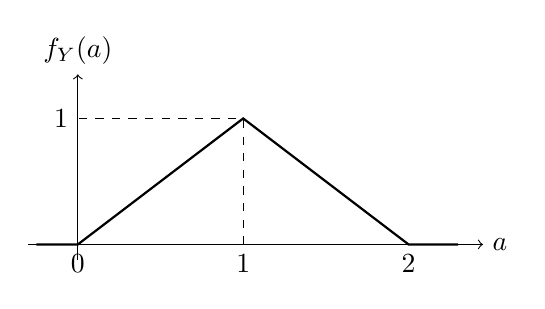
\begin{tikzpicture}[x=2.1cm,y=1.6cm]
\draw[->] (-.3,0)--(2.45,0) node[right] {$a$};
\draw[->] (0,-.12)--(0,1.35) node[above] {$f_Y(a)$};
\draw[thick] (-.25,0)--(0,0)--(1,1)--(2,0)--(2.3,0);
\draw[dashed] (1,0)--(1,1)--(0,1);
\node[below] at (0,0) {$0$};\node[below] at (1,0) {$1$};\node[below] at (2,0) {$2$};\node[left] at (0,1) {$1$};
\end{tikzpicture}
\end{center}
\end{solution}

\begin{exercise}\label{m2:2012f:q3}
2012年秋季原题3 (20分). $X_1,\ldots,X_n$ 为相互独立的 $[0,1]$ 均匀变量, $n$ 为正整数.
\begin{enumerate}
\item[(a)]\phantomsection\label{m2:2012f:q3:a} 令 $Y=\min\{X_1,\ldots,X_n\}$. 求 $a\in[0,1]$ 时的CDF $F_Y(a)$ 与密度 $f_Y(a)$.
\item[(b)]\phantomsection\label{m2:2012f:q3:b} 求 $\Prob(X_1<0.3)$ 与 $\Prob(\max\{X_1,\ldots,X_n\}<0.3)$.
\item[(c)]\phantomsection\label{m2:2012f:q3:c} 求 $\E[X_1+\cdots+X_n]$.
\end{enumerate}
\end{exercise}
\begin{solution}
(a) 最小值大于 $a$ 需要全部变量都大于 $a$, 所以 $\Prob(Y>a)=(1-a)^n$ ($0\le a\le1$). 因而 $F_Y(a)=1-(1-a)^n$, 内点的导数是 $f_Y(a)=n(1-a)^{n-1}$. 补全实轴上CDF: $a<0$ 时为0, $a>1$ 时为1; 密度在区间外为0.

(b) 单个变量落在长度0.3的区间内的概率为0.3. 最大值小于0.3则要求全部变量都落在该区间内, 独立性给出概率 $(0.3)^n$.

(c) 每个均值为 $1/2$, 期望可加性给出 $n/2$. 此步骤只需期望可加性, 不必另外调用独立性.
\end{solution}

\begin{exercise}\label{m2:2012f:q4}
2012年秋季原题4 (20分). 编剧Rachel把自己锁在房间里构思剧本. 好点子出现时刻是速率每小时 $\lambda_G=0.5$ 的Poisson过程, 坏点子出现时刻是速率每小时 $\lambda_B=1.5$ 的Poisson过程. 原题未明确两过程独立; 为使官方的叠加解法成立, 本稿明确假设两过程相互独立.
\begin{enumerate}
\item[(a)]\phantomsection\label{m2:2012f:q4:a} 令 $T$ 为第一个点子 (好或坏) 出现前的时间, 写出其密度.
\item[(b)]\phantomsection\label{m2:2012f:q4:b} 第一小时恰出现三个坏点子的概率是多少?
\item[(c)]\phantomsection\label{m2:2012f:q4:c} 令 $S$ 为第五个好点子出现前的时间, 求 $\Var(S)$.
\item[(d)]\phantomsection\label{m2:2012f:q4:d} 前三小时一个点子都没有的概率是多少?
\end{enumerate}
\end{exercise}
\begin{solution}
(a) 独立叠加后总速率为 $0.5+1.5=2$, 所以 $T\sim\Exp(2)$, 密度为 $2\ee^{-2t}$ ($t\ge0$), 负半轴为0. 若不补独立条件, 不能仅从两个边缘过程推出这个首次到达分布.

(b) 一小时坏点子数服从 $\Pois(1.5)$, 故概率为 $\ee^{-1.5}(1.5)^3/3!$.

(c) 好点子的五个连续到达间隔独立, 每个服从 $\Exp(0.5)$, 方差均为 $1/(0.5)^2=4$. $S$ 是这五个间隔之和, 故 $\Var(S)=5\cdot4=20$ (小时的平方).

(d) 三小时总点子数服从 $\Pois(2\cdot3)=\Pois(6)$, 零次概率为 $\ee^{-6}$. 也可由 $\Prob(T>3)=\ee^{-2\cdot3}$ 得到.
\end{solution}

\begin{exercise}\label{m2:2012f:q5}
2012年秋季原题5 (20分). $(X,Y)$ 的联合密度为
\[
f(x,y)=\begin{cases}1/\pi,&x^2+y^2<1,\\0,&x^2+y^2\ge1.\end{cases}
\]
\begin{enumerate}
\item[(a)]\phantomsection\label{m2:2012f:q5:a} 求 $X$ 的边缘密度 $f_X$.
\item[(b)]\phantomsection\label{m2:2012f:q5:b} 求 $\E[X\mid Y=0.5]$.
\item[(c)]\phantomsection\label{m2:2012f:q5:c} 将 $\E[X^3Y^3]$ 写成二重积分, 无需显式求值.
\end{enumerate}
\end{exercise}
\begin{solution}
(a) 固定 $x$, 单位圆盘的竖直截面为 $-\sqrt{1-x^2}<y<\sqrt{1-x^2}$, 仅当 $|x|<1$ 时非空. 对联合密度积分得
\[
f_X(x)=\begin{cases}\dfrac{2\sqrt{1-x^2}}\pi,&-1\le x\le1,\\0,&\text{其他}.\end{cases}
\]
官方解答把支持写成 $-1\le x\le-1$, 这里更正右端点为1. 密度的积分为1, 因为截面面积的积分恰是圆盘面积 $\pi$ 再除以 $\pi$.

(b) 给定 $Y=0.5$, 由条件密度 $f_{X\mid Y=y}(x)=f(x,y)/f_Y(y)$, $X$ 在 $(-\sqrt{3}/2,\sqrt{3}/2)$ 上均匀分布. 此区间关于0对称, 故条件期望为0. 条件事件本身概率为0, 此处使用的是由联合密度确定的连续条件分布.

(c) 依期望积分公式, 可写为
\[
\E[X^3Y^3]=\int_{-1}^1\int_{-\sqrt{1-x^2}}^{\sqrt{1-x^2}}\frac{x^3y^3}{\pi}\dd y\dd x.
\]
范围内变量有界, 因而这个积分存在; 实际上关于 $y$ 的奇对称也使其值为0, 但题目只要求积分表达.
\end{solution}

\begin{exercise}\label{m2:2012f:q6}
2012年秋季原题6 (10分). $X,Y$ 为相互独立的正态随机变量, 均值都为1, 方差都为9.
\begin{enumerate}
\item[(a)]\phantomsection\label{m2:2012f:q6:a} 写出 $(X,Y)$ 的联合密度 $f$ 的明确公式.
\item[(b)]\phantomsection\label{m2:2012f:q6:b} 求 $\E[X^2]$ 和 $\E[X^2Y^2]$.
\end{enumerate}
\end{exercise}
\begin{solution}
(a) 两个边缘密度分别为 $(3\sqrt{2\pi})^{-1}\ee^{-(x-1)^2/18}$ 与同式的 $y$ 版本. 独立性允许相乘, 从而
\[
f(x,y)=\frac1{18\pi}\exp\left(-\frac{(x-1)^2+(y-1)^2}{18}\right),\qquad(x,y)\in\R^2.
\]
官方最后合并指数的式子误把两个平方之间写成减号; 其前面的乘积式正确. 两个非负平方都须以负号进入指数, 才能在两个方向都可积.

(b) 由方差恒等式 $\E[X^2]=\Var(X)+(\E[X])^2=9+1=10$. $X^2,Y^2$ 仍独立, 所以 $\E[X^2Y^2]=\E[X^2]\E[Y^2]=10^2=100$.
\end{solution}

\originalsection{2014年春季}
题卷: \href{https://ocw.mit.edu/courses/18-600-probability-and-random-variables-fall-2019/resources/mit18_600f19_mid2_2014/}{MIT官方题卷}; 解答: \href{https://ocw.mit.edu/courses/18-600-probability-and-random-variables-fall-2019/resources/mit18_600f19_mid2_2014_soln/}{MIT官方解答}. 解答据官方重构补齐推导; 第4题补明官方叠加所需的独立条件. 第5题官方只给公式而未画要求的图, 两图为本稿新增重绘. 第4题保留 $(a),(c),(c),(d)$ 的原标号.

\begin{exercise}\label{m2:2014s:q1}
2014年春季原题1 (20分). 独立投掷一枚有偏硬币, 每次正面概率为 $3/4$, 反面概率为 $1/4$. 若第 $i$ 次为正面则 $X_i=1$, 否则为0.
\begin{enumerate}
\item[(a)]\phantomsection\label{m2:2014s:q1:a} 求 $\E[X_1]$ 和 $\Var(X_1)$.
\item[(b)]\phantomsection\label{m2:2014s:q1:b} 求 $\Var(X_1+2X_2+3X_3+4X_4)$.
\item[(c)]\phantomsection\label{m2:2014s:q1:c} 令 $Y=\sum_{i=1}^{4800}X_i$ 为前4800次的正面数. 用正态分布近似 $\Prob(Y\ge3690)$, 可用 $\Phi$.
\end{enumerate}
\end{exercise}
\begin{solution}
(a) $X_1^2=X_1$, 所以 $\E[X_1]=3/4$, $\Var(X_1)=3/4-(3/4)^2=3/16$.

(b) 独立性使混合协方差消失, 系数则在方差中平方, 因此
\[
\Var(X_1+2X_2+3X_3+4X_4)=\frac3{16}(1^2+2^2+3^2+4^2)=\frac{90}{16}=\frac{45}8.
\]

(c) $Y\sim\Bin(4800,3/4)$, 均值为3600, 方差为 $4800\cdot3/16=900$, 标准差为30. 3690比均值高3个标准差, 故官方近似为 $1-\Phi(3)$. 若采用连续性修正, $Y\ge3690$ 的连续边界为3689.5, 对应 $1-\Phi(179/60)$.
\end{solution}

\begin{exercise}\label{m2:2014s:q2}
2014年春季原题2 (10分). 公平六面骰子投掷一次, 点数为 $X\in\{1,2,3,4,5,6\}$. 若 $X\in\{1,2,3\}$ 则 $Y=1$, 否则 $Y=0$.
\begin{enumerate}
\item[(a)]\phantomsection\label{m2:2014s:q2:a} 求 $\E[X\mid Y=0]$.
\item[(b)]\phantomsection\label{m2:2014s:q2:b} 求 $\Var(Y\mid X=2)$.
\end{enumerate}
\end{exercise}
\begin{solution}
(a) $Y=0$ 恰好表示 $X\in\{4,5,6\}$. 这三个值的条件概率均为 $1/3$, 故条件均值为 $(4+5+6)/3=5$.

(b) 给定 $X=2$, $Y$ 必为1, 条件分布退化为常数. 因而条件方差为 $1-1^2=0$.
\end{solution}

\begin{exercise}\label{m2:2014s:q3}
2014年春季原题3 (20分). $X$ 在集合 $\{-2,-1,0,1,2\}$ 上均匀分布, 每个值概率为 $1/5$. $Y$ 为与 $X$ 同分布且独立的变量, 令 $Z=X+Y$.
\begin{enumerate}
\item[(a)]\phantomsection\label{m2:2014s:q3:a} 求 $M_X(t)$.
\item[(b)]\phantomsection\label{m2:2014s:q3:b} 求 $M_Z(t)$.
\end{enumerate}
\end{exercise}
\begin{solution}
(a) 逐点对 $\ee^{tX}$ 求期望得 $M_X(t)=(\ee^{-2t}+\ee^{-t}+1+\ee^t+\ee^{2t})/5$, 对所有实数 $t$ 成立.

(b) 由于 $\ee^{tZ}=\ee^{tX}\ee^{tY}$ 且 $X,Y$ 独立,
\[
M_Z(t)=M_X(t)M_Y(t)=\left(\frac{\ee^{-2t}+\ee^{-t}+1+\ee^t+\ee^{2t}}5\right)^2.
\]
在 $t=0$ 两个矩母函数都为1, 与定义相符.
\end{solution}

\begin{exercise}\label{m2:2014s:q4}
2014年春季原题4 (20分). 狮子队与老虎队从时刻0开始一场无限长的足球赛. 狮子队进球时刻形成速率每小时 $\lambda_L=2$ 的Poisson过程, 老虎队进球时刻形成速率每小时 $\lambda_T=3$ 的Poisson过程. 原题未明说独立, 本稿按官方解法补充两过程相互独立.
\begin{enumerate}
\item[(a)]\phantomsection\label{m2:2014s:q4:a} 写出狮子队首次进球时间的密度.
\item[(c), 第1次]\phantomsection\label{m2:2014s:q4:c1} 写出任意一队首次进球时间的密度.
\item[(c), 第2次]\phantomsection\label{m2:2014s:q4:c2} 老虎队前两小时一个球也不进的概率是多少?
\item[(d)]\phantomsection\label{m2:2014s:q4:d} 狮子队第一小时恰进三球的概率是多少?
\end{enumerate}
\end{exercise}
\begin{solution}
(a) 狮子队首次进球前等待时间服从 $\Exp(2)$, 密度为 $2\ee^{-2t}$ ($t\ge0$), 在负半轴为0.

(c), 第1次. 任意队首次进球前, 两队都不能进球. 对 $t\ge0$, 生存概率为 $\ee^{-2t}\ee^{-3t}=\ee^{-5t}$. 因而所求密度为 $5\ee^{-5t}$ ($t\ge0$), 负半轴为0; 这里相乘用到了补明的独立性.

(c), 第2次. 两小时老虎队进球数服从 $\Pois(3\cdot2)=\Pois(6)$, 零球概率为 $\ee^{-6}$.

(d) 第一小时狮子队进球数服从 $\Pois(2)$, 恰三球概率为 $\ee^{-2}2^3/3!=4/(3\ee^2)$. 这是时间1小时和速率2的组合, 不能把两队总速率5代入.
\end{solution}

\begin{exercise}\label{m2:2014s:q5}
2014年春季原题5 (20分). $X,Y$ 为独立的 $[0,1]$ 均匀变量, 令 $Z=X+Y$, $W=\max\{X,Y\}$.
\begin{enumerate}
\item[(a)]\phantomsection\label{m2:2014s:q5:a} 求密度 $f_Z$ 并画图.
\item[(b)]\phantomsection\label{m2:2014s:q5:b} 求CDF $F_W$ 并画图.
\item[(c)]\phantomsection\label{m2:2014s:q5:c} 求 $\Var(X),\Var(Y),\Var(Z)$.
\item[(d)]\phantomsection\label{m2:2014s:q5:d} 求 $\Cov(Y,Z)$ 与 $\rho(Y,Z)$.
\end{enumerate}
\end{exercise}
\begin{solution}
(a) 固定和 $z$, 卷积积分中的可行 $y$ 满足 $0<y<1$ 与 $0<z-y<1$. 因而可行区间为 $(0,1)\cap(z-1,z)$, 其长度给出
\[
f_Z(z)=\begin{cases}z,&0\le z\le1,\\2-z,&1<z\le2,\\0,&\text{其他}.\end{cases}
\]
图像由 $(0,0),(1,1),(2,0)$ 三点的线段及两侧零线组成. 这一计算与2012年秋季原题2(d)一致, 此处为保持本题要求而给出图.

(b) $W\le w$ 当且仅当 $X,Y$ 都不超过 $w$. 因此 $0\le w\le1$ 时 $F_W(w)=w^2$, 完整CDF为
\[
F_W(w)=\begin{cases}0,&w<0,\\w^2,&0\le w\le1,\\1,&w>1.\end{cases}
\]
它从0连续上升到1, 区间外分别保持0和1.
\begin{center}
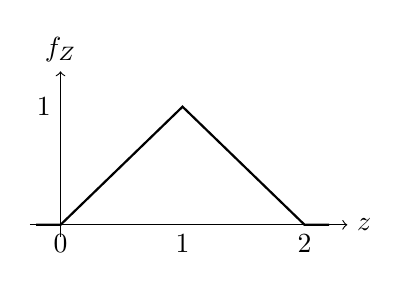
\begin{tikzpicture}[x=1.55cm,y=1.5cm]
\draw[->] (-.25,0)--(2.35,0) node[right] {$z$};\draw[->] (0,-.1)--(0,1.3) node[above] {$f_Z$};
\draw[thick] (-.2,0)--(0,0)--(1,1)--(2,0)--(2.2,0);
\node[below] at (0,0) {$0$};\node[below] at (1,0) {$1$};\node[below] at (2,0) {$2$};\node[left] at (0,1) {$1$};
\end{tikzpicture}\qquad
\begin{tikzpicture}[x=2.2cm,y=1.5cm]
\draw[->] (-.3,0)--(1.65,0) node[right] {$w$};\draw[->] (0,-.1)--(0,1.3) node[above] {$F_W$};
\draw[thick] (-.25,0)--(0,0);\draw[thick,domain=0:1,samples=50] plot (\x,{\x*\x});\draw[thick] (1,1)--(1.5,1);
\draw[dashed] (1,0)--(1,1)--(0,1);\node[below] at (0,0) {$0$};\node[below] at (1,0) {$1$};\node[left] at (0,1) {$1$};
\end{tikzpicture}
\end{center}

(c) 均匀变量满足 $\E[X]=1/2$, $\E[X^2]=1/3$, 所以 $\Var(X)=\Var(Y)=1/12$. 由独立性 $\Var(Z)=1/12+1/12=1/6$.

(d) $\Cov(Y,X+Y)=\Cov(Y,X)+\Var(Y)=1/12$, 因此
\[
\rho(Y,Z)=\frac{1/12}{\sqrt{(1/12)(1/6)}}=\frac1{\sqrt2}.
\]
虽 $X,Y$ 独立, $Y$ 与含有它的和 $Z$ 则正相关.
\end{solution}

\begin{exercise}\label{m2:2014s:q6}
2014年春季原题6 (10分). $X,Y$ 相互独立, 各服从速率 $\lambda=5$ 的指数分布.
\begin{enumerate}
\item[(a)]\phantomsection\label{m2:2014s:q6:a} 写出 $(X,Y)$ 联合密度的明确公式.
\item[(b)]\phantomsection\label{m2:2014s:q6:b} 求 $\E[X^2Y]$.
\end{enumerate}
\end{exercise}
\begin{solution}
(a) 独立性使联合密度为两个边缘密度的乘积:
\[
f(x,y)=\begin{cases}25\ee^{-5(x+y)},&x\ge0,\ y\ge0,\\0,&\text{其他}.\end{cases}
\]
正象限的支持不能省略, 否则负方向上的表达式不可积.

(b) $X^2$ 与 $Y$ 独立, $\E[Y]=1/5$. 对二阶矩作变量替换 $u=5x$:
\[
\E[X^2]=\int_0^\infty x^2\,5\ee^{-5x}\dd x=\frac1{25}\int_0^\infty u^2\ee^{-u}\dd u=\frac2{25}.
\]
最后一步可分部积分两次得到 $2!$. 因此 $\E[X^2Y]=(2/25)(1/5)=2/125$.
\end{solution}

\originalsection{2016年春季}
题卷: \href{https://ocw.mit.edu/courses/18-600-probability-and-random-variables-fall-2019/resources/mit18_600f19_mid2_2016/}{MIT官方题卷}; 解答: \href{https://ocw.mit.edu/courses/18-600-probability-and-random-variables-fall-2019/resources/mit18_600f19_mid2_2016_soln/}{MIT官方解答}. 本节据官方解答重构补齐, 特别区分Poisson过程速率与有限时段计数参数. 第6题调用标准柯西分布的稳定性, 同时给出特征函数上的理由.

\begin{exercise}\label{m2:2016s:q1}
2016年春季原题1 (20分). 一枚硬币每次正面概率为 $2/3$, 反面概率为 $1/3$, 各次投掷独立. 第 $i$ 次的正面指标为 $X_i$, 令 $S_n=\sum_{i=1}^nX_i$.
\begin{enumerate}
\item[(a)]\phantomsection\label{m2:2016s:q1:a} 求 $\E[X_1],\Var(X_1)$.
\item[(b)]\phantomsection\label{m2:2016s:q1:b} 将 $\E[S_n],\Var(S_n)$ 写成 $n$ 的函数.
\item[(c)]\phantomsection\label{m2:2016s:q1:c} 求 $\Cov(S_5,S_{10})$.
\item[(d)]\phantomsection\label{m2:2016s:q1:d} 用正态近似估计 $\Prob(S_{300}\le220)$, 可用 $\Phi$.
\end{enumerate}
\end{exercise}
\begin{solution}
(a) Bernoulli指标的均值为 $p=2/3$, 方差为 $p(1-p)=2/9$.

(b) 期望逐项相加, 方差由独立性逐项相加, 得 $\E[S_n]=2n/3$, $\Var(S_n)=2n/9$.

(c) 写 $S_{10}=S_5+(X_6+\cdots+X_{10})$. 后一部分与 $S_5$ 独立, 因而 $\Cov(S_5,S_{10})=\Var(S_5)=5\cdot2/9=10/9$. 也可双重求和 $\sum_{i=1}^5\sum_{j=1}^{10}\Cov(X_i,X_j)$, 只有 $i=j$ 的五项非零.

(d) $S_{300}$ 的均值为200, 方差为 $600/9$, 标准差为 $\sqrt{600/9}$. 官方使用阈值220, 得
\[
\Prob(S_{300}\le220)\approx\Phi\left(\frac{220-200}{\sqrt{600/9}}\right)=\Phi(\sqrt6).
\]
整数上界220采用连续性修正时, 可改用 $\Phi(20.5/\sqrt{600/9})$. 这里所求是累计下尾, 因而无需用 $1-\Phi$.
\end{solution}

\begin{exercise}\label{m2:2016s:q2}
2016年春季原题2 (20分). $X,Y$ 是两次独立公平骰子投掷的点数, 各在 $\{1,2,3,4,5,6\}$ 上均匀分布, 令 $Z=X+Y$.
\begin{enumerate}
\item[(a)]\phantomsection\label{m2:2016s:q2:a} 求 $X$ 的矩母函数.
\item[(b)]\phantomsection\label{m2:2016s:q2:b} 求 $Z$ 的矩母函数.
\item[(c)]\phantomsection\label{m2:2016s:q2:c} 求 $\E[Y\mid Z]$, 即将这个条件期望随机变量写成 $Z$ 的函数.
\end{enumerate}
\end{exercise}
\begin{solution}
(a) 每个点数概率为 $1/6$, 故 $M_X(t)=\frac16\sum_{k=1}^6\ee^{kt}$.

(b) 独立性使 $M_Z(t)=M_X(t)M_Y(t)=[\frac16\sum_{k=1}^6\ee^{kt}]^2$.

(c) 在给定 $Z=k$ 后, 可行点对 $(x,y)$ 与交换后的 $(y,x)$ 仍有相同概率. 所以 $\E[X\mid Z]=\E[Y\mid Z]$. 又由条件期望的线性性,
\[
\E[X\mid Z]+\E[Y\mid Z]=\E[X+Y\mid Z]=\E[Z\mid Z]=Z.
\]
故 $\E[Y\mid Z]=Z/2$ (几乎处处). 逐个取 $k=2,\ldots,12$ 也可验证: 给定和为 $k$, $Y$ 在 $\max(1,k-6)$ 至 $\min(6,k-1)$ 的连续整数上均匀分布, 两端的平均为 $k/2$.
\end{solution}

\begin{exercise}\label{m2:2016s:q3}
2016年春季原题3 (20分). $X$ 在 $[0,5]$ 上均匀分布, $Y$ 为独立的 $[0,10]$ 均匀变量, 令 $Z=\min\{X,Y\}$.
\begin{enumerate}
\item[(a)]\phantomsection\label{m2:2016s:q3:a} 求 $(X,Y)$ 的联合密度.
\item[(b)]\phantomsection\label{m2:2016s:q3:b} 求 $\Prob(Z>0),\Prob(Z>3),\Prob(Z>5)$.
\item[(c)]\phantomsection\label{m2:2016s:q3:c} 求CDF $F_Z(a)$.
\end{enumerate}
\end{exercise}
\begin{solution}
(a) 矩形 $[0,5]\times[0,10]$ 内联合密度为 $(1/5)(1/10)=1/50$, 矩形外为0.

(b) 两个连续均匀变量都严格大于0的概率为1, 所以 $\Prob(Z>0)=1$. 由独立性,
\[
\Prob(Z>3)=\Prob(X>3)\Prob(Y>3)=\frac25\frac7{10}=\frac7{25}.
\]
因 $Z\le X\le5$ 几乎必然, $\Prob(Z>5)=0$.

(c) $0\le a\le5$ 时两个区间上的尾概率均非零, 故 $1-F_Z(a)=((5-a)/5)((10-a)/10)$. 完整公式为
\[
F_Z(a)=\begin{cases}0,&a<0,\\1-\dfrac{(5-a)(10-a)}{50},&0\le a\le5,\\1,&a>5.\end{cases}
\]
在0处中间式为0, 在5处为1, 与左右常数段连续相接; 在区间内单调增加.
\end{solution}

\begin{exercise}\label{m2:2016s:q4}
2016年春季原题4 (20分). Alice的糕点店从上午7点营业至晚上10点, 共900分钟. 顾客按速率每分钟 $\lambda=1$ 的Poisson过程到达, 即平均每分钟一位. 令 $N$ 为全天到达总数.
\begin{enumerate}
\item[(a)]\phantomsection\label{m2:2016s:q4:a} 前三分钟恰有三位顾客到达的概率是多少?
\item[(b)]\phantomsection\label{m2:2016s:q4:b} 写出从开店到第二位顾客到达的等待时间密度. 本问假定关店后顾客仍继续到达, 不必考虑900分钟的上界, 因而第二位顾客最终会以概率1到达.
\item[(c)]\phantomsection\label{m2:2016s:q4:c} 求 $\E[N],\Var(N)$.
\item[(d)]\phantomsection\label{m2:2016s:q4:d} 全天没有一位顾客到达的概率是多少?
\end{enumerate}
\end{exercise}
\begin{solution}
(a) 三分钟计数服从 $\Pois(\lambda t)=\Pois(3)$, 恰三位的概率为 $\ee^{-3}3^3/3!=(9/2)\ee^{-3}$.

(b) 第二个到达时刻是两个独立 $\Exp(1)$ 间隔之和, 所以为形状2、速率1的Gamma变量. 也可直接卷积得到, 对 $t\ge0$,
\[
f(t)=\int_0^t\ee^{-u}\ee^{-(t-u)}\dd u=t\ee^{-t};
\]
负半轴密度为0. 将过程延续到关店后, 排除了等待时间被截断的情形.

(c) 全天计数参数是 $\lambda\cdot900=900$, 因而 $N\sim\Pois(900)$, $\E[N]=\Var(N)=900$. 官方写 $\E[N]=\lambda=900$, 混用了原来速率1与时段计数参数900; 此处明确区分.

(d) 由 $\Pois(900)$ 的零次概率, 得 $\Prob(N=0)=\ee^{-900}$. 等价地, 第一次到达时间为 $\Exp(1)$, 超过900分钟的概率为 $\ee^{-900}$.
\end{solution}

\begin{exercise}\label{m2:2016s:q5}
2016年春季原题5 (10分). $X_1,\ldots,X_n$ 相互独立, 各服从速率 $\lambda=1$ 的指数分布.
\begin{enumerate}
\item[(a)]\phantomsection\label{m2:2016s:q5:a} 令 $Y=\min\{X_1,\ldots,X_n\}$, 求密度 $f_Y$.
\item[(b)]\phantomsection\label{m2:2016s:q5:b} 将 $\E[Y^k]$ 写成 $n,k$ 的函数, 可假设 $n,k$ 均为正整数.
\end{enumerate}
\end{exercise}
\begin{solution}
(a) 对 $y\ge0$, 全部变量超过 $y$ 的概率为 $\ee^{-ny}$, 所以 $Y\sim\Exp(n)$, 密度为 $n\ee^{-ny}$ ($y\ge0$), 负半轴为0.

(b) 将 $u=ny$ 代入矩积分,
\[
\E[Y^k]=\int_0^\infty y^k n\ee^{-ny}\dd y=\frac1{n^k}\int_0^\infty u^k\ee^{-u}\dd u=\frac{k!}{n^k}.
\]
最后一个积分记为 $I_k$. 分部积分给出 $I_k=kI_{k-1}$, $I_0=1$; 边界项 $u^k\ee^{-u}$ 在0和无穷处都为0 ($k\ge1$), 因而 $I_k=k!$. 这同时说明矩有限, 并解释了 $n^{-k}$ 的缩放.
\end{solution}

\begin{exercise}\label{m2:2016s:q6}\phantomsection\label{m2:2016s:q6:whole}
2016年春季原题6 (10分). $X_1,\ldots,X_n$ 相互独立, 各自的密度为 $f(x)=1/[\pi(1+x^2)]$ ($x\in\R$). 求 $\Prob(X_1+\cdots+X_n\ge n)$.
\end{exercise}
\begin{solution}
每个变量服从标准柯西分布. 柯西稳定性表明平均值 $A=n^{-1}\sum_iX_i$ 仍是标准柯西变量. 在特征函数层面, 标准柯西的特征函数是 $\ee^{-|t|}$; 用独立性可核验
\[
\varphi_A(t)=\prod_{i=1}^n\varphi_{X_i}(t/n)=(\ee^{-|t|/n})^n=\ee^{-|t|}.
\]
由特征函数决定分布, 这给出所用稳定性结论. 所求事件等价于 $A\ge1$, 而柯西变量没有点质量, 因而
\[
\Prob(A\ge1)=\int_1^\infty\frac{\dd x}{\pi(1+x^2)}=\frac1\pi\left(\frac\pi2-\arctan1\right)=\frac14.
\]
柯西变量的均值与方差不存在, 所以此题不能套用有限方差中心极限定理. 特征函数论证是对官方稳定性解法的本稿补充, 并未把样本平均误作趋于常数.
\end{solution}

\originalsection{2017年春季}
题卷: \href{https://ocw.mit.edu/courses/18-600-probability-and-random-variables-fall-2019/resources/mit18_600f19_mid2_2017/}{MIT官方题卷}; 解答: \href{https://ocw.mit.edu/courses/18-600-probability-and-random-variables-fall-2019/resources/mit18_600f19_mid2_2017_soln/}{MIT官方解答}. 本节依官方答案补齐推导, 明确修正密度记号、缩放公式与Beta归一化常数的笔误. 原题2的第二问印作 ``b)'', 本稿保留其字母 $b$.

\begin{exercise}\label{m2:2017s:q1}
2017年春季原题1 (10分). $X,Y,Z$ 相互独立, 各以概率 $1/3$ 取值1, 以概率 $2/3$ 取值5. 令 $W=X+Y+Z$.
\begin{enumerate}
\item[(a)]\phantomsection\label{m2:2017s:q1:a} 求矩母函数 $M_X$.
\item[(b)]\phantomsection\label{m2:2017s:q1:b} 求矩母函数 $M_W$.
\end{enumerate}
\end{exercise}
\begin{solution}
(a) 根据两点的概率加权, 得 $M_X(t)=\frac13\ee^t+\frac23\ee^{5t}$, 对所有实数 $t$ 成立.

(b) 独立性使和的矩母函数为三个因子的乘积, 因此 $M_W(t)=(\frac13\ee^t+\frac23\ee^{5t})^3$. 特别地 $M_W(0)=1$, 而 $M_W'(0)=3\E[X]=11$, 与三个同分布变量的期望之和一致.
\end{solution}

\begin{exercise}\label{m2:2017s:q2}
2017年春季原题2 (15分). $X_1,\ldots,X_7$ 为相互独立的标准正态变量, 各均值0、方差1, 令 $Z=\sum_{j=1}^7X_j$.
\begin{enumerate}
\item[(a)]\phantomsection\label{m2:2017s:q2:a} 给出 $Z$ 的概率密度.
\item[(b)]\phantomsection\label{m2:2017s:q2:b} 求 $\Prob(X_1<X_2<\cdots<X_7)$.
\end{enumerate}
\end{exercise}
\begin{solution}
(a) 独立正态变量之和仍为正态, 其均值与方差分别相加, 故 $Z\sim\Normal(0,7)$. 密度为
\[
f_Z(z)=\frac1{\sqrt{14\pi}}\ee^{-z^2/14},\qquad z\in\R.
\]
官方把这一密度误记作 $F_Z$; 本稿采用小写 $f_Z$ 与CDF区别.

(b) 连续分布保证任意两变量相等的概率为0. 因为变量独立且同分布, 对下标任意置换都不改变联合分布, 所以 $7!$ 种严格排列有相同概率. 这些事件互斥且合计概率1, 故指定顺序的概率为 $1/7!$.
\end{solution}

\begin{exercise}\label{m2:2017s:q3}
2017年春季原题3 (15分). $X_1,X_2,X_3$ 相互独立, 各服从速率 $\lambda=1$ 的指数分布.
\begin{enumerate}
\item[(a)]\phantomsection\label{m2:2017s:q3:a} 求 $\min\{X_1,X_2,X_3\}$ 的密度.
\item[(b)]\phantomsection\label{m2:2017s:q3:b} 求 $\E[\max\{X_1,X_2,X_3\}]$.
\end{enumerate}
\end{exercise}
\begin{solution}
(a) 最小值超过 $t\ge0$ 的概率是 $\ee^{-t}\ee^{-t}\ee^{-t}=\ee^{-3t}$, 所以其密度为 $3\ee^{-3t}$ ($t\ge0$), 负半轴为0.

(b) 采用相邻次序统计量之间的间隔. 第一段等到三个中首个发生, 速率为3; 发生后利用无记忆性, 剩余两个寿命独立且仍为 $\Exp(1)$, 故第二段速率2; 最后一段速率1. 最大值是三段之和, 因而期望为 $1/3+1/2+1=11/6$. 这与习题\ref{m2:2011s:q4}取 $\lambda=1$ 的特例一致.
\end{solution}

\begin{exercise}\label{m2:2017s:q4}
2017年春季原题4 (10分). $X,Y$ 相互独立, 各具有密度 $f(x)=1/[\pi(1+x^2)]$ ($x\in\R$).
\begin{enumerate}
\item[(a)]\phantomsection\label{m2:2017s:q4:a} 求 $A=(X+Y)/2$ 的密度.
\item[(b)]\phantomsection\label{m2:2017s:q4:b} 求 $B=X-Y$ 的密度.
\end{enumerate}
\end{exercise}
\begin{solution}
(a) 两个标准柯西变量的平均仍为标准柯西. 用特征函数验证为 $\varphi_A(t)=\ee^{-|t|/2}\ee^{-|t|/2}=\ee^{-|t|}$. 所以 $f_A(a)=1/[\pi(1+a^2)]$ ($a\in\R$).

(b) 标准柯西密度关于0对称, 因而 $-Y$ 与 $Y$ 同分布, 且仍与 $X$ 独立. 所以 $B$ 与 $X+Y=2A$ 同分布. 对连续变量缩放, 变量代换中的Jacobian为 $1/2$, 从而
\[
f_B(b)=\frac12 f_A(b/2)=\frac1{2\pi(1+(b/2)^2)}=\frac2{\pi(4+b^2)}.
\]
官方中间式写成 $\frac12 f_B(b/2)$, 应为 $\frac12 f_A(b/2)$; 其最终明确密度正确. 在此 $B$ 的尺度为2, 不可仍使用尺度1的密度.
\end{solution}

\begin{exercise}\label{m2:2017s:q5}
2017年春季原题5 (15分). $C$ 表示一个很大群体中, 被询问时更喜欢咖喱而非披萨的学生比例. 起初对 $C$ 一无所知, 以 $[0,1]$ 均匀分布为Bayes先验. 从群体中均匀抽取一名学生询问偏好, 再独立重复两次. 三个回答中两人偏好咖喱, 一人偏好披萨.
\begin{enumerate}
\item[(a)]\phantomsection\label{m2:2017s:q5:a} 根据这三个回答, 求未知比例 $C$ 的后验密度 $f_C$.
\item[(b)]\phantomsection\label{m2:2017s:q5:b} 先验下 $\E[C]=1/2$. 得知三个回答后, $C$ 的期望应修正为多少?
\end{enumerate}
可使用: Beta$(a,b)$ 的均值为 $a/(a+b)$, 密度为 $x^{a-1}(1-x)^{b-1}/B(a,b)$; 对正整数 $a,b$, $B(a,b)=(a-1)!(b-1)!/(a+b-1)!$.
\end{exercise}
\begin{solution}
(a) 给定 $C=c$, 三次独立询问得到两咖喱一披萨的似然与 $c^2(1-c)$ 成正比. 若记录的是人数而非指定回答顺序, 似然前多一个系数3; 它与 $c$ 无关, 会在归一化时消去. 先验密度为1, 所以后验密度为
\[
f_C(c\mid\text{回答})=\frac{c^2(1-c)}{\int_0^1u^2(1-u)\dd u}=12c^2(1-c),\qquad0\le c\le1,
\]
区间外为0. 分母等于 $1/3-1/4=1/12=B(3,2)$, 故后验是Beta$(3,2)$. 官方将归一化一行误写为乘以 $B(2,3)$; 此处更正为除以 $B(3,2)$.

(b) 由给定Beta均值公式, 后验均值为 $3/(3+2)=3/5$. 直接积分也得 $12\int_0^1c^3(1-c)\dd c=12(1/4-1/5)=3/5$, 与参数公式一致.
\end{solution}

\begin{exercise}\label{m2:2017s:q6}
2017年春季原题6 (15分). $X_1,\ldots,X_{100}$ 相互独立, 各以概率 $1/2$ 取1, 以概率 $1/2$ 取0. 令 $S=\sum_{j=1}^{100}X_j$.
\begin{enumerate}
\item[(a)]\phantomsection\label{m2:2017s:q6:a} 求 $\E[S],\Var(S)$.
\item[(b)]\phantomsection\label{m2:2017s:q6:b} 用正态近似估计 $\Prob(S>60)$, 可用 $\Phi$.
\end{enumerate}
\end{exercise}
\begin{solution}
(a) $S\sim\Bin(100,1/2)$, 均值为 $100/2=50$, 方差为 $100(1/2)(1/2)=25$.

(b) 标准差为5, 60比均值高两个标准差. 官方不作连续性修正时给出 $\Prob(S>60)\approx1-\Phi(2)=\Phi(-2)$. 精确整数事件为 $S\ge61$, 若作连续性修正, 阈值为60.5, 得到 $1-\Phi(2.1)$. 两式估计的是同一个离散尾事件, 差异来自连续边界的选择.
\end{solution}

\begin{exercise}\label{m2:2017s:q7}
2017年春季原题7 (20分). 某行星居民谨慎使用核武器, 但区域性核战争仍发生. 战争时刻构成速率为每千年1次的Poisson点过程, 因而任意1000年期内战争数的期望为1.
\begin{enumerate}
\item[(a)]\phantomsection\label{m2:2017s:q7:a} 接下来2000年恰有三场核战争的概率是多少?
\item[(b)]\phantomsection\label{m2:2017s:q7:b} 令 $X$ 为第三场核战争前的千年数, 即 $1000X$ 为所需年数. 求其密度 $f_X$.
\item[(c)]\phantomsection\label{m2:2017s:q7:c} 令 $Y$ 为接下来5000年的核战争数, 求 $\Var(Y)$.
\end{enumerate}
\end{exercise}
\begin{solution}
(a) 以千年为时间单位, 2000年对应时长2, 战争数服从 $\Pois(2)$. 恰三场的概率为 $\ee^{-2}2^3/3!=4/(3\ee^2)$.

(b) 同样以千年计, 每个到达间隔服从 $\Exp(1)$. 第三次到达是三个独立间隔之和, 为形状3、速率1的Gamma变量, 密度为 $f_X(x)=x^2\ee^{-x}/2$ ($x\ge0$), 在 $x<0$ 时为0. 若误用每年的速率 $1/1000$ 却仍把横轴记成千年, 会改变该密度的尺度.

(c) 五千年计数服从 $\Pois(5)$, Poisson分布的方差等于其参数, 故 $\Var(Y)=5$.
\end{solution}

\originalsection{2018年春季}
题卷: \href{https://ocw.mit.edu/courses/18-600-probability-and-random-variables-fall-2019/resources/mit18_600f19_mid2_2018/}{MIT官方题卷}; 解答: \href{https://ocw.mit.edu/courses/18-600-probability-and-random-variables-fall-2019/resources/mit18_600f19_mid2_2018_soln/}{MIT官方解答}. 本节据官方答案补齐主计算链; 第5题原联合密度指数及极坐标Jacobian的笔误明示更正, 第7题补上特征函数零点值.

\begin{exercise}\label{m2:2018s:q1}
2018年春季原题1 (20分). $X$ 的密度为
\[
f(x)=\begin{cases}x/2,&0<x\le2,\\0,&x\le0\text{ 或 }x>2.\end{cases}
\]
$Y$ 是与 $X$ 同分布且独立的变量, 令 $Z=X^2+Y^2$.
\begin{enumerate}
\item[(a)]\phantomsection\label{m2:2018s:q1:a} 求联合密度 $f_{X,Y}(x,y)$.
\item[(b)]\phantomsection\label{m2:2018s:q1:b} 求 $\E[Z]$, 给出明确数值.
\item[(c)]\phantomsection\label{m2:2018s:q1:c} 求 $\Prob(\max\{X,Y\}\le1)$.
\end{enumerate}
\end{exercise}
\begin{solution}
(a) 先核对 $\int_0^2x/2\dd x=1$, 因而边缘密度归一化. 独立性给出联合密度 $xy/4$ ($0<x\le2,0<y\le2$), 矩形外为0.

(b) 两变量同分布, 期望相加给出
\[
\E[Z]=2\E[X^2]=2\int_0^2x^2\frac x2\dd x=\int_0^2x^3\dd x=\left[\frac{x^4}4\right]_0^2=4.
\]
这个求和步骤不需要先求 $Z$ 的密度.

(c) 最大值不超过1表示两变量都不超过1. 各自概率为 $\int_0^1x/2\dd x=1/4$, 所以独立性给出 $\Prob(\max\{X,Y\}\le1)=(1/4)^2=1/16$.
\end{solution}

\begin{exercise}\label{m2:2018s:q2}
2018年春季原题2 (10分). 某群体中有 $n=110000$ 名健康人, 每人在给定十年中以概率 $p=0.01$ 罹患某疾病, 各人的事件相互独立. $X$ 为患病人数.
\begin{enumerate}
\item[(a)]\phantomsection\label{m2:2018s:q2:a} 求 $\E[X],\Var(X)$.
\item[(b)]\phantomsection\label{m2:2018s:q2:b} 用正态近似估计 $\Prob(1100<X<1133)$, 可用 $\Phi$.
\end{enumerate}
\end{exercise}
\begin{solution}
(a) $X\sim\Bin(110000,0.01)$, 均值为1100, 方差为 $110000(0.01)(0.99)=1089=33^2$.

(b) 标准差33, 两个连续阈值1100与1133分别对应标准化后的0、1. 官方近似为 $\Phi(1)-\Phi(0)$. 原整数事件为 $1101\le X\le1132$, 连续性修正后区间为 $(1100.5,1132.5)$, 故另可估为 $\Phi(65/66)-\Phi(1/66)$. 不应将严格上下界直接当作包含端点的整数事件.
\end{solution}

\begin{exercise}\label{m2:2018s:q3}
2018年春季原题3 (20分). $X_1,X_2,X_3$ 相互独立, 密度均为 $f(x)=\ee^{-x}$ ($x\ge0$), 在 $x<0$ 时为0. 令 $X=X_1+X_2+X_3$, $A=\min\{X_1,X_2,X_3\}$, $B=\max\{X_1,X_2,X_3\}$.
\begin{enumerate}
\item[(a)]\phantomsection\label{m2:2018s:q3:a} 求 $X$ 的密度.
\item[(b)]\phantomsection\label{m2:2018s:q3:b} 求 $A$ 的密度.
\item[(c)]\phantomsection\label{m2:2018s:q3:c} 求 $\E[B]$ 与 $\Var(B)$.
\end{enumerate}
\end{exercise}
\begin{solution}
(a) 三个变量均为 $\Exp(1)$, 和服从形状3、速率1的Gamma分布. 明确密度为 $f_X(x)=x^2\ee^{-x}/2$ ($x\ge0$), 负半轴为0. 可先卷积前两个得 $t\ee^{-t}$, 再卷积第三个:
\[
f_X(x)=\int_0^x t\ee^{-t}\ee^{-(x-t)}\dd t=\ee^{-x}\frac{x^2}2,\qquad x\ge0.
\]

(b) $\Prob(A>a)=\ee^{-3a}$ ($a\ge0$), 所以 $f_A(a)=3\ee^{-3a}$ ($a\ge0$), 负半轴为0.

(c) 按衰变先后分解 $B=D_1+D_2+D_3$. 第一段 $D_1\sim\Exp(3)$; 利用无记忆性, 后续剩余寿命分布不依赖此前已经等待的时长, 故 $D_2\sim\Exp(2)$、$D_3\sim\Exp(1)$ 且三个间隔独立. 因而不仅均值可以相加, 方差也可以相加:
\[
\E[B]=\frac13+\frac12+1=\frac{11}6,\qquad
\Var(B)=\frac1{3^2}+\frac1{2^2}+1=\frac{49}{36}.
\]
方差计算中的独立对象是相邻次序统计量增量, 原来的最小值、最大值并不独立.
\end{solution}

\begin{exercise}\label{m2:2018s:q4}
2018年春季原题4 (10分). $X,Y,Z$ 相互独立, 各具有标准柯西密度 $f(x)=1/[\pi(1+x^2)]$. 令 $V=3X$, $W=X+Y+Z$.
\begin{enumerate}
\item[(a)]\phantomsection\label{m2:2018s:q4:a} 求 $V$ 的密度.
\item[(b)]\phantomsection\label{m2:2018s:q4:b} 求 $W$ 的密度.
\end{enumerate}
\end{exercise}
\begin{solution}
(a) 由于 $F_V(v)=F_X(v/3)$, 求导得到 $f_V(v)=\frac13f_X(v/3)=1/[3\pi(1+(v/3)^2)]=3/[\pi(9+v^2)]$, 对整个实轴成立.

(b) 独立性给出 $\varphi_W(t)=(\ee^{-|t|})^3=\ee^{-3|t|}=\varphi_V(t)$, 所以 $W,V$ 同分布. 因而 $f_W(w)=3/[\pi(9+w^2)]$. 这说明三变量之和尺度为3, 与三倍单变量具有相同分布, 但并非随机变量逐点相等.
\end{solution}

\begin{exercise}\label{m2:2018s:q5}
2018年春季原题5 (10分). $X,Y$ 相互独立, 各为均值0、方差1的标准正态变量.
\begin{enumerate}
\item[(a)]\phantomsection\label{m2:2018s:q5:a} 求 $\Prob(X^2+Y^2\le1)$, 给出明确值.
\item[(b)]\phantomsection\label{m2:2018s:q5:b} 求 $\Prob(\max\{|X|,|Y|\}\le1)$, 可用 $\Phi$.
\end{enumerate}
\end{exercise}
\begin{solution}
(a) 联合密度为 $(2\pi)^{-1}\ee^{-(x^2+y^2)/2}$. 原官方第一行误写指数 $-x^2-y^2$, 随后的极坐标式又漏写Jacobian $r$; 本稿按正态边缘密度的乘积修正. 在单位圆盘上令 $x=r\cos\theta,y=r\sin\theta$, 面积元素为 $r\dd r\dd\theta$. 因而
\begin{align*}
\Prob(X^2+Y^2\le1)
&=\int_0^1\int_0^{2\pi}\frac1{2\pi}\ee^{-r^2/2}r\dd\theta\dd r\\
&=\int_0^1r\ee^{-r^2/2}\dd r
=\left[-\ee^{-r^2/2}\right]_0^1=1-\ee^{-1/2}.
\end{align*}
(b) 所求事件为 $|X|\le1$ 与 $|Y|\le1$ 同时成立, 是正方形而不是圆盘. 每个一维概率为 $\Phi(1)-\Phi(-1)$, 独立性给出 $[\Phi(1)-\Phi(-1)]^2=[2\Phi(1)-1]^2$.
\end{solution}

\begin{exercise}\label{m2:2018s:q6}
2018年春季原题6 (20分). $X,Y$ 独立且均在 $[0,1]$ 上均匀分布, 令 $Z=X+Y$.
\begin{enumerate}
\item[(a)]\phantomsection\label{m2:2018s:q6:a} 求 $\E[X\mid Z]$, 将其写成 $Z$ 的函数.
\item[(b)]\phantomsection\label{m2:2018s:q6:b} 求 $\E[Z\mid X]$, 将其写成 $X$ 的函数.
\item[(c)]\phantomsection\label{m2:2018s:q6:c} 求 $\Var(Z\mid Y)$, 将其写成 $Y$ 的函数.
\item[(d)]\phantomsection\label{m2:2018s:q6:d} 求 $\rho(X,Z)$.
\end{enumerate}
\end{exercise}
\begin{solution}
(a) 联合分布在交换 $X,Y$ 后不变, 给定和也不破坏这种对称性, 所以 $\E[X\mid Z]=\E[Y\mid Z]$. 又两者之和为 $\E[X+Y\mid Z]=Z$, 故 $\E[X\mid Z]=Z/2$. 这与双骰子题使用相同的可交换性, 但本题的变量分布不同, 不合并题面.

(b) 条件期望的线性性给出 $\E[Z\mid X]=\E[X\mid X]+\E[Y\mid X]$. 第一项为 $X$, 独立性使第二项为常数 $\E[Y]=1/2$, 所以结果是 $X+1/2$.

(c) 给定 $Y=y$, $Z$ 在 $[y,y+1]$ 上均匀分布. 平移不改变方差, 因此 $\Var(Z\mid Y)=1/12$ 几乎处处. 亦可计算条件中心化量 $Z-\E[Z\mid Y]=X-1/2$, 其条件二阶矩为 $\E[(X-1/2)^2]=1/12$.

(d) $\Cov(X,Z)=\Cov(X,X+Y)=\Var(X)=1/12$, $\Var(Z)=\Var(X)+\Var(Y)=1/6$. 所以 $\rho(X,Z)=(1/12)/\sqrt{(1/12)(1/6)}=1/\sqrt2$.
\end{solution}

\begin{exercise}\label{m2:2018s:q7}
2018年春季原题7 (10分). $X_1,\ldots,X_n$ 为相互独立的 $[0,1]$ 均匀变量, 令 $X=\sum_{j=1}^nX_j$.
\begin{enumerate}
\item[(a)]\phantomsection\label{m2:2018s:q7:a} 求特征函数 $\varphi_{X_1}(t)$.
\item[(b)]\phantomsection\label{m2:2018s:q7:b} 求特征函数 $\varphi_X(t)$.
\end{enumerate}
\end{exercise}
\begin{solution}
(a) 特征函数使用 $\ee^{\ii tX_1}$ 而非实指数. 对 $t\ne0$,
\[
\varphi_{X_1}(t)=\int_0^1\ee^{\ii tx}\dd x=\frac{\ee^{\ii t}-1}{\ii t}.
\]
当 $t=0$ 时, 被积函数为1, 所以 $\varphi_{X_1}(0)=1$. 该值也等于商式的极限, 不能把零点排除而称其为完整特征函数.

(b) 各变量独立且同分布, 因而
\[
\varphi_X(t)=\begin{cases}\left(\dfrac{\ee^{\ii t}-1}{\ii t}\right)^n,&t\ne0,\\1,&t=0.\end{cases}
\]
复指数的模恒为1, 故这些期望对每个实数 $t$ 都存在, 无需额外矩存在条件.
\end{solution}

\originalsection{2019年春季}
题卷: \href{https://ocw.mit.edu/courses/18-600-probability-and-random-variables-fall-2019/resources/mit18_600f19_mid2_2019/}{MIT官方题卷}; 解答: \href{https://ocw.mit.edu/courses/18-600-probability-and-random-variables-fall-2019/resources/mit18_600f19_mid2_2019_soln/}{MIT官方解答}. 本节依据官方答案重构补齐推导. 第2题补明三过程共同独立, 第6题修正条件密度零分支的支持笔误; 第7题CDF负半轴与边界属于本稿补全.

\begin{exercise}\label{m2:2019s:q1}
2019年春季原题1 (10分). Ramona参加篮球罚球比赛, 共投100球. 每球独立地以概率0.8命中、概率0.2未中. $X$ 为命中总数.
\begin{enumerate}
\item[(a)]\phantomsection\label{m2:2019s:q1:a} 求 $X$ 的期望与方差.
\item[(b)]\phantomsection\label{m2:2019s:q1:b} 用正态变量估计她共命中76至84球的概率, 可用 $\Phi$.
\end{enumerate}
\end{exercise}
\begin{solution}
(a) $X\sim\Bin(100,0.8)$, 均值 $np=80$, 方差 $np(1-p)=16$, 所以标准差为4.

(b) 官方将76与84看作均值两侧各一个标准差的阈值, 得到 $\Phi(1)-\Phi(-1)\approx0.68$. 原文 ``between 76 and 84'' 未声明是否包含端点; 官方未作连续性修正, 对这两种整数约定都采用相同连续阈值近似. 若理解为包含端点的 $76\le X\le84$, 连续性修正边界为75.5与84.5, 近似为 $\Phi(9/8)-\Phi(-9/8)$. 若理解为严格介于两者之间, 则事件为 $77\le X\le83$, 边界为76.5与83.5, 修正近似为 $\Phi(7/8)-\Phi(-7/8)$. 题面歧义不影响(a)的精确结果.
\end{solution}

\begin{exercise}\label{m2:2019s:q2}
2019年春季原题2 (20分). Becky的百吉饼店生意繁忙, 顾客随机到达, 每位顾客立即购买一种百吉饼. 肉桂葡萄干百吉饼出售时刻 $C_1,C_2,\ldots$ 构成每分钟速率1的Poisson过程, 黑麦百吉饼出售时刻 $P_1,P_2,\ldots$ 构成速率2的独立Poisson过程, 综合口味百吉饼出售时刻 $E_1,E_2,\ldots$ 构成速率3的Poisson过程. 原题对第三个过程的共同独立性未完整明说; 本稿按官方解答补明三过程相互独立.
\begin{enumerate}
\item[(a)]\phantomsection\label{m2:2019s:q2:a} 求 $C_3$ 的密度.
\item[(b)]\phantomsection\label{m2:2019s:q2:b} 求 $X=\min\{C_1,P_1,E_1\}$ 的密度.
\item[(c)]\phantomsection\label{m2:2019s:q2:c} 开店前两分钟总共恰售出10个百吉饼的概率是多少?
\item[(d)]\phantomsection\label{m2:2019s:q2:d} 求 $\E[\cos(P_1+E_1^2)]$, 可留作二重积分, 无需求值.
\end{enumerate}
\end{exercise}
\begin{solution}
(a) $C_3$ 是三个独立 $\Exp(1)$ 间隔之和, 密度为 $c^2\ee^{-c}/2$ ($c\ge0$), 负半轴为0, 即形状3、速率1的Gamma分布.

(b) 前 $t$ 分钟没有任何类型售出的概率为 $\ee^{-t}\ee^{-2t}\ee^{-3t}=\ee^{-6t}$. 故 $X\sim\Exp(6)$, 密度为 $6\ee^{-6x}$ ($x\ge0$), 负半轴为0.

(c) 叠加过程速率为 $1+2+3=6$, 两分钟计数服从 $\Pois(12)$. 所求概率为 $\ee^{-12}12^{10}/10!$.

(d) 首次黑麦售出时间 $P_1\sim\Exp(2)$, 首次综合口味售出时间 $E_1\sim\Exp(3)$, 二者独立. 对 $x,y\ge0$ 联合密度为 $6\ee^{-2x-3y}$, 故
\[
\E[\cos(P_1+E_1^2)]=\int_0^\infty\int_0^\infty6\ee^{-2x-3y}\cos(x+y^2)\dd x\dd y.
\]
余弦绝对值不超过1, 密度积分为1, 所以积分绝对收敛, 允许任选这两个积分的次序.
\end{solution}

\begin{exercise}\label{m2:2019s:q3}
2019年春季原题3 (10分). 实随机变量 $(X,Y)$ 的联合密度为
\[
f(x,y)=\frac1{\pi^2(1+x^2)(1+y^2)},\qquad(x,y)\in\R^2.
\]
\begin{enumerate}
\item[(a)]\phantomsection\label{m2:2019s:q3:a} 求 $(X+Y)/2$ 的密度.
\item[(b)]\phantomsection\label{m2:2019s:q3:b} 求 $\Prob(X>Y+2)$.
\end{enumerate}
\end{exercise}
\begin{solution}
(a) 联合密度分解为两个各自积分为1的标准柯西密度, 所以 $X,Y$ 独立且均为标准柯西. 其平均 $A=(X+Y)/2$ 的特征函数为 $\ee^{-|t|/2}\ee^{-|t|/2}=\ee^{-|t|}$, 故 $f_A(a)=1/[\pi(1+a^2)]$ ($a\in\R$).

(b) 对称性使 $-Y$ 与 $Y$ 同分布且仍与 $X$ 独立, 所以 $(X-Y)/2$ 也为标准柯西. 事件 $X>Y+2$ 等价于 $(X-Y)/2>1$, 因而
\[
\Prob(X>Y+2)=\int_1^\infty\frac{\dd u}{\pi(1+u^2)}=\frac14.
\]
官方中途换成 $(X+Y)/2>1$ 时依靠的是同分布, 不是两个事件逐点相同; 这里将事件等价与概率因同分布相等分开说明.
\end{solution}

\begin{exercise}\label{m2:2019s:q4}
2019年春季原题4 (20分). $X_1,X_2,X_3,X_4$ 相互独立, 密度均为 $(2\pi)^{-1/2}\ee^{-x^2/2}$, 即标准正态密度.
\begin{enumerate}
\item[(a)]\phantomsection\label{m2:2019s:q4:a} 求 $\rho(X_1+X_2+X_3,X_2+X_3+X_4)$.
\item[(b)]\phantomsection\label{m2:2019s:q4:b} 求 $\Prob(\min\{X_1,X_2\}>\max\{X_3,X_4\})$.
\item[(c)]\phantomsection\label{m2:2019s:q4:c} 求 $X_1+X_2+X_3$ 的密度.
\item[(d)]\phantomsection\label{m2:2019s:q4:d} 求 $\Prob(X_1^2+X_3^2\le2)$, 给出明确值.
\end{enumerate}
\end{exercise}
\begin{solution}
(a) 不同下标的协方差为0, 同下标的协方差为1. 展开两个和的协方差, 仅共同的 $X_2,X_3$ 各贡献1, 所以协方差为2. 两个和的方差均为3, 因而相关系数为 $2/\sqrt{3\cdot3}=2/3$.

(b) 所求事件表示 $X_1,X_2$ 是最大的两项, 不限制这两项内部以及另外两项内部的顺序. 连续同分布变量有 $4!$ 种等可能严格顺序, 符合条件的有 $2!2!=4$ 种, 所以概率为 $4/24=1/6$. 也可把最大的两项下标看作 $\binom42=6$ 个等可能的二元集合之一.

(c) 三个独立标准正态之和为 $\Normal(0,3)$, 因而密度为 $f(s)=(6\pi)^{-1/2}\ee^{-s^2/6}$ ($s\in\R$). 分母的尺度 $\sqrt3$ 来自标准差, 不是方差3本身.

(d) $X_1,X_3$ 的联合密度为 $(2\pi)^{-1}\ee^{-(x^2+y^2)/2}$. 所求区域为半径 $\sqrt2$ 的圆盘. 极坐标代换给出
\begin{align*}
\Prob(X_1^2+X_3^2\le2)
&=\int_0^{\sqrt2}\int_0^{2\pi}\frac1{2\pi}\ee^{-r^2/2}r\dd\theta\dd r\\
&=\left[-\ee^{-r^2/2}\right]_0^{\sqrt2}=1-\ee^{-1}.
\end{align*}
圆周本身概率为0, 所以将不等号写为严格小于也不改变结果.
\end{solution}

\begin{exercise}\label{m2:2019s:q5}
2019年春季原题5 (10分). $A,B,C,D$ 相互独立, 均在 $[0,1]$ 上均匀分布. 后来得知 $A$ 是四者中的第三大.
\begin{enumerate}
\item[(a)]\phantomsection\label{m2:2019s:q5:a} 根据这个新信息, 求 $A$ 的修正密度 (Bayes后验).
\item[(b)]\phantomsection\label{m2:2019s:q5:b} 先验下 $\E[A]=1/2$. 得知 $A$ 为第三大后, 修正后的期望是多少?
\end{enumerate}
可使用Beta$(a,b)$的均值 $a/(a+b)$ 与密度 $x^{a-1}(1-x)^{b-1}/B(a,b)$, 其中 $B(a,b)=(a-1)!(b-1)!/(a+b-1)!$ (正整数参数).
\end{exercise}
\begin{solution}
(a) 四者中的第三大等于第二小, 所以恰有一项小于 $A$, 两项大于 $A$. 给定 $A=a$, 其余三项独立, 恰一个小于 $a$ 的概率为 $3a(1-a)^2$. 先验密度为1, 事件 ``$A$为第三大'' 的概率为 $1/4$, 所以条件密度为
\[
f_{A\mid\text{第三大}}(a)=\frac{3a(1-a)^2}{1/4}=12a(1-a)^2,\qquad0\le a\le1,
\]
区间外为0. 这是Beta$(2,3)$, 因 $B(2,3)=1!2!/4!=1/12$. 此处区分第三大与第三小很关键: 后者会交换两个参数.

(b) 由Beta均值公式, 条件期望为 $2/(2+3)=2/5$. 直接积分为 $12\int_0^1a^2(1-a)^2\dd a=12(1/3-1/2+1/5)=2/5$. 比先验均值略低, 与其为第二小相符.
\end{solution}

\begin{exercise}\label{m2:2019s:q6}
2019年春季原题6 (15分). $(X,Y)$ 在三角形 $T=\{(x,y):x\ge0,y\ge0,x+y\le1\}$ 上均匀分布, 即 $f_{X,Y}(x,y)=2$ ($(x,y)\in T$), 三角形外为0.
\begin{enumerate}
\item[(a)]\phantomsection\label{m2:2019s:q6:a} 求边缘密度 $f_X$.
\item[(b)]\phantomsection\label{m2:2019s:q6:b} 求 $\Prob(X<2Y)$.
\item[(c)]\phantomsection\label{m2:2019s:q6:c} 求条件密度 $f_{X\mid Y=0.5}(x)$.
\end{enumerate}
\end{exercise}
\begin{solution}
(a) 对 $x\in[0,1]$, 竖直截面为 $0\le y\le1-x$, 故 $f_X(x)=\int_0^{1-x}2\dd y=2(1-x)$. 区间外为0. 积分 $\int_0^12(1-x)\dd x=1$, 确认边缘归一化.

(b) 直线 $x=2y$ 与斜边 $x+y=1$ 相交于 $(2/3,1/3)$. 满足 $x<2y$ 的部分是顶点 $(0,0),(0,1),(2/3,1/3)$ 的三角形, 面积为 $\frac12\cdot1\cdot\frac23=1/3$. 整个 $T$ 面积为1/2, 联合密度恒定, 所以概率为 $(1/3)/(1/2)=2/3$. 以下图中阴影是所求区域, 直线边界对概率无贡献.
\begin{center}
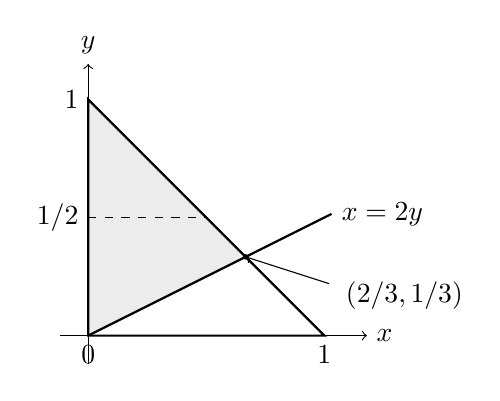
\begin{tikzpicture}[x=3cm,y=3cm]
\fill[gray!15] (0,0)--(0,1)--(2/3,1/3)--cycle;
\draw[->] (-.12,0)--(1.18,0) node[right] {$x$};\draw[->] (0,-.12)--(0,1.15) node[above] {$y$};
\draw[thick] (0,0)--(1,0)--(0,1)--cycle;
\draw[thick] (0,0)--(1.03,.515) node[right] {$x=2y$};
\fill (2/3,1/3) circle (1pt);\draw[->] (1.02,.22)--(2/3,1/3);\node[right] at (1.05,.17) {$(2/3,1/3)$};
\draw[dashed] (0,.5)--(.5,.5);\node[left] at (0,.5) {$1/2$};
\node[below] at (0,0) {$0$};\node[below] at (1,0) {$1$};\node[left] at (0,1) {$1$};
\end{tikzpicture}
\end{center}

(c) 对称性给出 $f_Y(y)=2(1-y)$ ($0\le y\le1$), 所以 $f_Y(1/2)=1$. 固定 $y=1/2$ 后支持为 $0\le x\le1/2$, 因而
\[
f_{X\mid Y=1/2}(x)=\frac{f_{X,Y}(x,1/2)}{f_Y(1/2)}=\begin{cases}2,&0\le x\le1/2,\\0,&\text{其他}.\end{cases}
\]
官方零分支误写 $x\notin[0,2]$, 本稿更正为 $x\notin[0,1/2]$. 条件密度的积分为 $2\cdot1/2=1$, 与水平截面上的均匀分布相符.
\end{solution}

\begin{exercise}\label{m2:2019s:q7}
2019年春季原题7 (15分). $X\sim\Exp(1)$, 令 $Z=X^5$.
\begin{enumerate}
\item[(a)]\phantomsection\label{m2:2019s:q7:a} 将CDF $F_Z(a)$ 写成 $a$ 的函数.
\item[(b)]\phantomsection\label{m2:2019s:q7:b} 求 $\E[Z^2]$.
\item[(c)]\phantomsection\label{m2:2019s:q7:c} 求 $\Prob(Z>32\mid Z>1)$.
\end{enumerate}
\end{exercise}
\begin{solution}
(a) $X\ge0$ 几乎必然, 所以 $Z\ge0$. 在非负半轴五次幂严格递增, 因而
\[
F_Z(a)=\begin{cases}0,&a<0,\\\Prob(X\le a^{1/5})=1-\ee^{-a^{1/5}},&a\ge0.\end{cases}
\]
官方只写非负部分, 此处补齐负半轴. $a=0$ 时CDF为0, $a\to\infty$ 时趋于1.

(b) $Z^2=X^{10}$, 故 $\E[Z^2]=\int_0^\infty x^{10}\ee^{-x}\dd x=10!$. 分部积分递推 $I_k=kI_{k-1}$、$I_0=1$ 给出此结果, 不是 $(\E[Z])^2=(5!)^2$.

(c) 因 $32=2^5$、$1=1^5$, 事件转换为 $X>2$ 给定 $X>1$. 用指数尾函数相除得
\[
\Prob(Z>32\mid Z>1)=\frac{\ee^{-2}}{\ee^{-1}}=\ee^{-1}.
\]
这正是无记忆性 $\Prob(X>1+1\mid X>1)=\Prob(X>1)$.
\end{solution}

\originalsection{2019年秋季}
题卷: \href{https://ocw.mit.edu/courses/18-600-probability-and-random-variables-fall-2019/resources/mit18_600f19_midterm2/}{MIT官方题卷}; 解答: \href{https://ocw.mit.edu/courses/18-600-probability-and-random-variables-fall-2019/resources/mit18_600f19_midterm2_soln/}{MIT官方解答}. 本节依据官方解答补齐推导. 原题5与2011年春季原题5整题相同, 保留逐子问映射而不重复习题. 原题6的题卷密度不归一, 下文明示其原式, 再采用官方解答的归一化版本求解.

\begin{exercise}\label{m2:2019f:q1}
2019年秋季原题1 (20分).
\begin{enumerate}
\item[(a)]\phantomsection\label{m2:2019f:q1:a} Melissa向20所外州医学院申请. 她的GPA、MCAT成绩与申请文书很优秀, 每所学校以概率 $1/20$ 录取她, 各校决定独立. 用Poisson近似估计至少两所录取的概率.
\item[(b)]\phantomsection\label{m2:2019f:q1:b} Jill向25所外州医学院申请, 独立地以概率 $1/5$ 得到每所学校的面试邀请. $X$ 为邀请她面试的学校数. 求 $\E[X],\Var(X)$.
\item[(c)]\phantomsection\label{m2:2019f:q1:c} 用正态近似粗略估计Jill得到少于2.5所学校面试邀请的概率, 可用 $\Phi$.
\end{enumerate}
\end{exercise}
\begin{solution}
(a) 录取数 $A\sim\Bin(20,1/20)$, $np=1$. 用参数1的Poisson变量近似, 得
\[
\Prob(A\ge2)\approx1-\Prob(\Pois(1)=0)-\Prob(\Pois(1)=1)=1-\frac2\ee\approx0.26424.
\]
精确二项概率为 $1-(19/20)^{20}-20(1/20)(19/20)^{19}\approx0.26416$, 所以此处近似很好. 这项数值比较来自官方解答, 不将Poisson近似写成精确概率.

(b) $X\sim\Bin(25,1/5)$, 均值为5, 方差为 $25(1/5)(4/5)=4$.

(c) 标准差为2, 2.5比均值低 $5/4$ 个标准差, 故正态近似为 $\Phi((2.5-5)/2)=\Phi(-5/4)\approx0.10565$. 因 $X$ 为整数, $X<2.5$ 等价于 $X\le2$, 2.5本身已是这个事件的连续性修正边界. 精确值为 $\sum_{k=0}^2\binom{25}k(1/5)^k(4/5)^{25-k}\approx0.098$, 与官方比较一致.
\end{solution}

\begin{exercise}\label{m2:2019f:q2}
2019年秋季原题2 (20分). 房间有四只灯泡, 寿命 $X_1,X_2,X_3,X_4$ 相互独立且均为速率1的指数变量. 令
\[
X=X_1+X_2+X_3+X_4,\quad Y=\min\{X_1,X_2,X_3,X_4\},\quad Z=\max\{X_1,X_2,X_3,X_4\}.
\]
$Y$ 为首只灯泡烧坏时刻, $Z$ 为最后一只烧坏时刻.
\begin{enumerate}
\item[(a)]\phantomsection\label{m2:2019f:q2:a} 求 $f_X$.
\item[(b)]\phantomsection\label{m2:2019f:q2:b} 求 $f_Y$.
\item[(c)]\phantomsection\label{m2:2019f:q2:c} 求 $\E[Z]$.
\item[(d)]\phantomsection\label{m2:2019f:q2:d} 求 $\Cov(Y,Z)$. 提示: 使用无记忆性.
\end{enumerate}
\end{exercise}
\begin{solution}
(a) 四个独立 $\Exp(1)$ 之和为形状4、速率1的Gamma变量, 所以 $f_X(x)=x^3\ee^{-x}/3!$ ($x\ge0$), 负半轴为0. 一般连续卷积递推将 $x^{k-1}\ee^{-x}/(k-1)!$ 积分一次, 得 $x^k\ee^{-x}/k!$, 这里取四个间隔.

(b) $\Prob(Y>y)=\prod_{j=1}^4\Prob(X_j>y)=\ee^{-4y}$ ($y\ge0$), 所以 $Y\sim\Exp(4)$, 密度为 $4\ee^{-4y}$ ($y\ge0$), 负半轴为0.

(c) 将最后烧坏时刻分成四段相邻烧坏时刻之间的间隔. 活着的灯泡数依次为4、3、2、1, 每次烧坏后剩余寿命依无记忆性仍为独立 $\Exp(1)$. 四段的速率分别为4、3、2、1, 因而 $\E[Z]=1/4+1/3+1/2+1=25/12$.

(d) 第一个烧坏后, 其余三灯泡的剩余寿命分布不随首个等待时间 $Y$ 变化. 因而 $Z-Y$ (剩余三只全部烧坏的等待时间) 与 $Y$ 独立. 首次烧坏的是哪一只不影响此条件分布, 所以该独立性在不指定灯泡下标时仍成立. 协方差展开得
\[
\Cov(Y,Z)=\Cov(Y,Y+(Z-Y))=\Var(Y)+\Cov(Y,Z-Y)=\Var(Y)=\frac1{4^2}=\frac1{16}.
\]
最小寿命与最大寿命并不独立; 独立的是最小寿命与随后经历的时间增量.
\end{solution}

\begin{exercise}\label{m2:2019f:q3}
2019年秋季原题3 (20分). 五位求职者的面试分数 $X_1,\ldots,X_5$ 为独立同分布的 $[0,1]$ 均匀变量. 最高分为 $Y=\max\{X_1,\ldots,X_5\}$, 次高分 $Z$ 为五个分数的第二大.
\begin{enumerate}
\item[(a)]\phantomsection\label{m2:2019f:q3:a} 求 $r\in[0,1]$ 时的 $F_Y(r)$.
\item[(b)]\phantomsection\label{m2:2019f:q3:b} 求 $f_Y$.
\item[(c)]\phantomsection\label{m2:2019f:q3:c} 求 $f_Z$ 与 $\E[Z]$. 可用Beta$(a,b)$均值 $a/(a+b)$、密度 $x^{a-1}(1-x)^{b-1}/B(a,b)$, 正整数参数时 $B(a,b)=(a-1)!(b-1)!/(a+b-1)!$.
\item[(d)]\phantomsection\label{m2:2019f:q3:d} 求 $\Prob(X_2>2X_1)$, 即第二位求职者分数超过第一位的两倍的概率.
\end{enumerate}
\end{exercise}
\begin{solution}
(a) $Y\le r$ 需要五项都不超过 $r$, 所以 $F_Y(r)=r^5$ ($0\le r\le1$). 区间左侧为0、右侧为1.

(b) 在区间内求导得 $f_Y(r)=5r^4$ ($0<r<1$), 其他地方为0, 端点密度可任意赋值而不改分布.

(c) 次高分不超过 $z$ 表示最多一项超过 $z$. 对 $z\in[0,1]$, 分成零项超过与恰一项超过两个互斥事件, 得
\[
F_Z(z)=z^5+5(1-z)z^4=5z^4-4z^5.
\]
求导得 $f_Z(z)=20z^3(1-z)$ ($0\le z\le1$), 区间外为0. 它为Beta$(4,2)$, $B(4,2)=3!1!/5!=1/20$. 均值为 $4/(4+2)=2/3$, 也可直接算 $20\int_0^1z^4(1-z)\dd z=20(1/5-1/6)=2/3$. 官方将该期望误记成 $\E[X]$, 本稿更正变量为 $Z$.

(d) 注意 $X_2$ 是第二位求职者的分数, 不等于次高分 $Z$. $(X_1,X_2)$ 在单位正方形上联合密度为1. 所求区域为 $0\le x<1/2$, $2x<y\le1$, 所以
\[
\Prob(X_2>2X_1)=\int_0^{1/2}\int_{2x}^1\dd y\dd x=\int_0^{1/2}(1-2x)\dd x=\frac14.
\]
其余三位分数对这一事件没有影响.
\end{solution}

\begin{exercise}\label{m2:2019f:q4}
2019年秋季原题4 (15分). $X,Y$ 相互独立, 各具有密度 $f(x)=1/[\pi(1+x^2)]$.
\begin{enumerate}
\item[(a)]\phantomsection\label{m2:2019f:q4:a} 求 $\Prob(X<1)$.
\item[(b)]\phantomsection\label{m2:2019f:q4:b} 求 $Z=(X-Y)/2$ 的密度.
\item[(c)]\phantomsection\label{m2:2019f:q4:c} 求 $\E[\ee^{-X^2-Y^2}]$, 可留作二重积分, 无需明确求值.
\end{enumerate}
\end{exercise}
\begin{solution}
(a) 由标准柯西CDF积分,
\[
\Prob(X<1)=\frac1\pi\int_{-\infty}^1\frac{\dd x}{1+x^2}=\frac1\pi\left(\arctan1+\frac\pi2\right)=\frac34.
\]
连续分布在1处没有点质量, 严格与非严格不等号结果相同.

(b) $-Y$ 仍为标准柯西且与 $X$ 独立. 因此 $Z$ 为两个独立标准柯西的平均, 特征函数为 $\ee^{-|t|}$, 密度是 $f_Z(z)=1/[\pi(1+z^2)]$ ($z\in\R$).

(c) 联合密度为 $[\pi^2(1+x^2)(1+y^2)]^{-1}$, 期望积分为
\[
\E[\ee^{-X^2-Y^2}]=\int_{-\infty}^{\infty}\int_{-\infty}^{\infty}\frac{\ee^{-x^2-y^2}}{\pi^2(1+x^2)(1+y^2)}\dd x\dd y.
\]
被积函数非负且不超过联合密度, 因而积分有限. 也可由独立性写成 $[\int_{\R}\ee^{-x^2}/(\pi(1+x^2))\dd x]^2$, 但题目只要求二重积分.
\end{solution}

\begin{remark}\label{m2:2019f:q5}
2019年秋季原题5 (10分) 与2011年春季原题5完全相同, 已在习题\ref{m2:2011s:q5}完整给出题面与解答. 原题 $X_1$ 对应该题 $X$, 原题十枚独立标准骰子之和 $S$ 对应该题 $Y$. 逐问映射为:
\begin{enumerate}
\item[(a)]\phantomsection\label{m2:2019f:q5:a} 原问 $M_{X_1}(t)$ 对应2011年春季Q5(a), 见习题\ref{m2:2011s:q5}的(a).
\item[(b)]\phantomsection\label{m2:2019f:q5:b} 原问 $M_S(t)$ 对应2011年春季Q5(b), 见习题\ref{m2:2011s:q5}的(b).
\end{enumerate}
两问的投掷次数、点数集合、各点概率与独立条件均相同, 因此这里保留原题来源与映射, 不重复设立习题.
\end{remark}

\begin{exercise}\label{m2:2019f:q6}
2019年秋季原题6 (15分). 题卷原印联合密度 $\widetilde f(x,y)=(2\pi)^{-1}\ee^{-x^2-y^2}$ ($x,y\in\R$), 但该函数积分为 $1/2$, 不是概率密度. 官方解答采用的是两个独立标准正态变量的归一化密度
\[
f_{X,Y}(x,y)=\frac1{2\pi}\ee^{-(x^2+y^2)/2},\qquad(x,y)\in\R^2.
\]
本题按官方解答的这个更正版求解, 令 $Z=X+Y$.
\begin{enumerate}
\item[(a)]\phantomsection\label{m2:2019f:q6:a} 求 $\E[XY]$.
\item[(b)]\phantomsection\label{m2:2019f:q6:b} 求 $\E[Y\mid Z]$, 写成 $Z$ 的函数.
\item[(c)]\phantomsection\label{m2:2019f:q6:c} 求 $\Prob(X^2+Y^2\le4)$.
\end{enumerate}
\end{exercise}
\begin{solution}
先核实勘误: $\int_{\R}\ee^{-x^2}\dd x=\sqrt\pi$, 所以原式总积分为 $(2\pi)^{-1}(\sqrt\pi)^2=1/2$. 将原式简单乘2会产生方差 $1/2$ 的正态边缘, 与官方答案不同; 本稿采用官方给出的指数除以2的更正, 并非暗中将原函数归一化为另一道题.

(a) 更正后的联合密度分解为两个标准正态密度, 所以 $X,Y$ 独立且均值0. 因此 $\E[XY]=\E[X]\E[Y]=0$. 也可对联合密度乘 $xy$ 后利用奇对称得到0; 正态变量二阶矩有限, 保证该期望存在.

(b) 对换 $X,Y$ 不改变联合分布, 给定 $Z=X+Y$ 后仍有 $\E[X\mid Z]=\E[Y\mid Z]$. 两者之和为 $\E[Z\mid Z]=Z$, 故 $\E[Y\mid Z]=Z/2$ 几乎处处.

(c) 区域为半径2的圆盘. 用 $x=r\cos\theta,y=r\sin\theta$ 和面积元素 $r\dd r\dd\theta$, 得
\begin{align*}
\Prob(X^2+Y^2\le4)
&=\int_0^2\int_0^{2\pi}\frac1{2\pi}\ee^{-r^2/2}r\dd\theta\dd r\\
&=\int_0^2r\ee^{-r^2/2}\dd r=\left[-\ee^{-r^2/2}\right]_0^2
=1-\ee^{-2}\approx0.86466.
\end{align*}
这与官方更正版本的答案一致; 若仅把原函数乘2归一化, 会得到 $1-\ee^{-4}$, 所以更正方式必须明示.
\end{solution}
